% Created 2024-08-16 Fri 23:01
% Intended LaTeX compiler: pdflatex
\documentclass[11pt]{article}
\usepackage[utf8]{inputenc}
\usepackage[T1]{fontenc}
\usepackage{graphicx}
\usepackage{grffile}
\usepackage{longtable}
\usepackage{wrapfig}
\usepackage{rotating}
\usepackage[normalem]{ulem}
\usepackage{amsmath}
\usepackage{textcomp}
\usepackage{amssymb}
\usepackage{capt-of}
\usepackage{hyperref}
\usepackage{amssymb}


\usepackage{algorithm}
\usepackage{multirow}

%
\usepackage{paralist}
\usepackage{makeidx}  % allows for indexgeneration
%
%\mainmatter           % start of the contributions
%
%

%\pagestyle{headings}  % switches on printing of running heads



\usepackage{color}
\definecolor{snow}{rgb}{1.000,0.980,0.980}
\definecolor{GhostWhite}{rgb}{0.973,0.973,1.000}
\definecolor{WhiteSmoke}{rgb}{0.961,0.961,0.961}
\definecolor{gainsboro}{rgb}{0.863,0.863,0.863}
\definecolor{FloralWhite}{rgb}{1.000,0.980,0.941}
\definecolor{OldLace}{rgb}{0.992,0.961,0.902}
\definecolor{linen}{rgb}{0.980,0.941,0.902}
\definecolor{AntiqueWhite}{rgb}{0.980,0.922,0.843}
\definecolor{PapayaWhip}{rgb}{1.000,0.937,0.835}
\definecolor{BlanchedAlmond}{rgb}{1.000,0.922,0.804}
\definecolor{bisque}{rgb}{1.000,0.894,0.769}
\definecolor{PeachPuff}{rgb}{1.000,0.855,0.725}
\definecolor{NavajoWhite}{rgb}{1.000,0.871,0.678}
\definecolor{moccasin}{rgb}{1.000,0.894,0.710}
\definecolor{cornsilk}{rgb}{1.000,0.973,0.863}
\definecolor{ivory}{rgb}{1.000,1.000,0.941}
\definecolor{LemonChiffon}{rgb}{1.000,0.980,0.804}
\definecolor{seashell}{rgb}{1.000,0.961,0.933}
\definecolor{honeydew}{rgb}{0.941,1.000,0.941}
\definecolor{MintCream}{rgb}{0.961,1.000,0.980}
\definecolor{azure}{rgb}{0.941,1.000,1.000}
\definecolor{AliceBlue}{rgb}{0.941,0.973,1.000}
\definecolor{lavender}{rgb}{0.902,0.902,0.980}
\definecolor{LavenderBlush}{rgb}{1.000,0.941,0.961}
\definecolor{MistyRose}{rgb}{1.000,0.894,0.882}
\definecolor{white}{rgb}{1.000,1.000,1.000}
\definecolor{black}{rgb}{0.000,0.000,0.000}
\definecolor{DarkSlateGray}{rgb}{0.184,0.310,0.310}
\definecolor{DarkSlateGrey}{rgb}{0.184,0.310,0.310}
\definecolor{DimGray}{rgb}{0.412,0.412,0.412}
\definecolor{DimGrey}{rgb}{0.412,0.412,0.412}
\definecolor{SlateGray}{rgb}{0.439,0.502,0.565}
\definecolor{SlateGrey}{rgb}{0.439,0.502,0.565}
\definecolor{LightSlateGray}{rgb}{0.467,0.533,0.600}
\definecolor{LightSlateGrey}{rgb}{0.467,0.533,0.600}
\definecolor{gray}{rgb}{0.745,0.745,0.745}
\definecolor{grey}{rgb}{0.745,0.745,0.745}
\definecolor{LightGrey}{rgb}{0.827,0.827,0.827}
\definecolor{LightGray}{rgb}{0.827,0.827,0.827}
\definecolor{MidnightBlue}{rgb}{0.098,0.098,0.439}
\definecolor{navy}{rgb}{0.000,0.000,0.502}
\definecolor{NavyBlue}{rgb}{0.000,0.000,0.502}
\definecolor{CornflowerBlue}{rgb}{0.392,0.584,0.929}
\definecolor{DarkSlateBlue}{rgb}{0.282,0.239,0.545}
\definecolor{SlateBlue}{rgb}{0.416,0.353,0.804}
\definecolor{MediumSlateBlue}{rgb}{0.482,0.408,0.933}
\definecolor{LightSlateBlue}{rgb}{0.518,0.439,1.000}
\definecolor{MediumBlue}{rgb}{0.000,0.000,0.804}
\definecolor{RoyalBlue}{rgb}{0.255,0.412,0.882}
\definecolor{blue}{rgb}{0.000,0.000,1.000}
\definecolor{DodgerBlue}{rgb}{0.118,0.565,1.000}
\definecolor{DeepSkyBlue}{rgb}{0.000,0.749,1.000}
\definecolor{SkyBlue}{rgb}{0.529,0.808,0.922}
\definecolor{LightSkyBlue}{rgb}{0.529,0.808,0.980}
\definecolor{SteelBlue}{rgb}{0.275,0.510,0.706}
\definecolor{LightSteelBlue}{rgb}{0.690,0.769,0.871}
\definecolor{LightBlue}{rgb}{0.678,0.847,0.902}
\definecolor{PowderBlue}{rgb}{0.690,0.878,0.902}
\definecolor{PaleTurquoise}{rgb}{0.686,0.933,0.933}
\definecolor{DarkTurquoise}{rgb}{0.000,0.808,0.820}
\definecolor{MediumTurquoise}{rgb}{0.282,0.820,0.800}
\definecolor{turquoise}{rgb}{0.251,0.878,0.816}
\definecolor{cyan}{rgb}{0.000,1.000,1.000}
\definecolor{LightCyan}{rgb}{0.878,1.000,1.000}
\definecolor{CadetBlue}{rgb}{0.373,0.620,0.627}
\definecolor{MediumAquamarine}{rgb}{0.400,0.804,0.667}
\definecolor{aquamarine}{rgb}{0.498,1.000,0.831}
\definecolor{DarkGreen}{rgb}{0.000,0.392,0.000}
\definecolor{DarkOliveGreen}{rgb}{0.333,0.420,0.184}
\definecolor{DarkSeaGreen}{rgb}{0.561,0.737,0.561}
\definecolor{SeaGreen}{rgb}{0.180,0.545,0.341}
\definecolor{MediumSeaGreen}{rgb}{0.235,0.702,0.443}
\definecolor{LightSeaGreen}{rgb}{0.125,0.698,0.667}
\definecolor{PaleGreen}{rgb}{0.596,0.984,0.596}
\definecolor{SpringGreen}{rgb}{0.000,1.000,0.498}
\definecolor{LawnGreen}{rgb}{0.486,0.988,0.000}
\definecolor{green}{rgb}{0.000,1.000,0.000}
\definecolor{chartreuse}{rgb}{0.498,1.000,0.000}
\definecolor{MediumSpringGreen}{rgb}{0.000,0.980,0.604}
\definecolor{GreenYellow}{rgb}{0.678,1.000,0.184}
\definecolor{LimeGreen}{rgb}{0.196,0.804,0.196}
\definecolor{YellowGreen}{rgb}{0.604,0.804,0.196}
\definecolor{ForestGreen}{rgb}{0.133,0.545,0.133}
\definecolor{OliveDrab}{rgb}{0.420,0.557,0.137}
\definecolor{DarkKhaki}{rgb}{0.741,0.718,0.420}
\definecolor{khaki}{rgb}{0.941,0.902,0.549}
\definecolor{PaleGoldenrod}{rgb}{0.933,0.910,0.667}
\definecolor{LightGoldenrodYellow}{rgb}{0.980,0.980,0.824}
\definecolor{LightYellow}{rgb}{1.000,1.000,0.878}
\definecolor{yellow}{rgb}{1.000,1.000,0.000}
\definecolor{gold}{rgb}{1.000,0.843,0.000}
\definecolor{LightGoldenrod}{rgb}{0.933,0.867,0.510}
\definecolor{goldenrod}{rgb}{0.855,0.647,0.125}
\definecolor{DarkGoldenrod}{rgb}{0.722,0.525,0.043}
\definecolor{RosyBrown}{rgb}{0.737,0.561,0.561}
\definecolor{IndianRed}{rgb}{0.804,0.361,0.361}
\definecolor{SaddleBrown}{rgb}{0.545,0.271,0.075}
\definecolor{sienna}{rgb}{0.627,0.322,0.176}
\definecolor{peru}{rgb}{0.804,0.522,0.247}
\definecolor{burlywood}{rgb}{0.871,0.722,0.529}
\definecolor{beige}{rgb}{0.961,0.961,0.863}
\definecolor{wheat}{rgb}{0.961,0.871,0.702}
\definecolor{SandyBrown}{rgb}{0.957,0.643,0.376}
\definecolor{tan}{rgb}{0.824,0.706,0.549}
\definecolor{chocolate}{rgb}{0.824,0.412,0.118}
\definecolor{firebrick}{rgb}{0.698,0.133,0.133}
\definecolor{brown}{rgb}{0.647,0.165,0.165}
\definecolor{DarkSalmon}{rgb}{0.914,0.588,0.478}
\definecolor{salmon}{rgb}{0.980,0.502,0.447}
\definecolor{LightSalmon}{rgb}{1.000,0.627,0.478}
\definecolor{orange}{rgb}{1.000,0.647,0.000}
\definecolor{DarkOrange}{rgb}{1.000,0.549,0.000}
\definecolor{coral}{rgb}{1.000,0.498,0.314}
\definecolor{LightCoral}{rgb}{0.941,0.502,0.502}
\definecolor{tomato}{rgb}{1.000,0.388,0.278}
\definecolor{OrangeRed}{rgb}{1.000,0.271,0.000}
\definecolor{red}{rgb}{1.000,0.000,0.000}
\definecolor{HotPink}{rgb}{1.000,0.412,0.706}
\definecolor{DeepPink}{rgb}{1.000,0.078,0.576}
\definecolor{pink}{rgb}{1.000,0.753,0.796}
\definecolor{LightPink}{rgb}{1.000,0.714,0.757}
\definecolor{PaleVioletRed}{rgb}{0.859,0.439,0.576}
\definecolor{maroon}{rgb}{0.690,0.188,0.376}
\definecolor{MediumVioletRed}{rgb}{0.780,0.082,0.522}
\definecolor{VioletRed}{rgb}{0.816,0.125,0.565}
\definecolor{magenta}{rgb}{1.000,0.000,1.000}
\definecolor{violet}{rgb}{0.933,0.510,0.933}
\definecolor{plum}{rgb}{0.867,0.627,0.867}
\definecolor{orchid}{rgb}{0.855,0.439,0.839}
\definecolor{MediumOrchid}{rgb}{0.729,0.333,0.827}
\definecolor{DarkOrchid}{rgb}{0.600,0.196,0.800}
\definecolor{DarkViolet}{rgb}{0.580,0.000,0.827}
\definecolor{BlueViolet}{rgb}{0.541,0.169,0.886}
\definecolor{purple}{rgb}{0.627,0.125,0.941}
\definecolor{MediumPurple}{rgb}{0.576,0.439,0.859}
\definecolor{thistle}{rgb}{0.847,0.749,0.847}
\definecolor{snow1}{rgb}{1.000,0.980,0.980}
\definecolor{snow2}{rgb}{0.933,0.914,0.914}
\definecolor{snow3}{rgb}{0.804,0.788,0.788}
\definecolor{snow4}{rgb}{0.545,0.537,0.537}
\definecolor{seashell1}{rgb}{1.000,0.961,0.933}
\definecolor{seashell2}{rgb}{0.933,0.898,0.871}
\definecolor{seashell3}{rgb}{0.804,0.773,0.749}
\definecolor{seashell4}{rgb}{0.545,0.525,0.510}
\definecolor{AntiqueWhite1}{rgb}{1.000,0.937,0.859}
\definecolor{AntiqueWhite2}{rgb}{0.933,0.875,0.800}
\definecolor{AntiqueWhite3}{rgb}{0.804,0.753,0.690}
\definecolor{AntiqueWhite4}{rgb}{0.545,0.514,0.471}
\definecolor{bisque1}{rgb}{1.000,0.894,0.769}
\definecolor{bisque2}{rgb}{0.933,0.835,0.718}
\definecolor{bisque3}{rgb}{0.804,0.718,0.620}
\definecolor{bisque4}{rgb}{0.545,0.490,0.420}
\definecolor{PeachPuff1}{rgb}{1.000,0.855,0.725}
\definecolor{PeachPuff2}{rgb}{0.933,0.796,0.678}
\definecolor{PeachPuff3}{rgb}{0.804,0.686,0.584}
\definecolor{PeachPuff4}{rgb}{0.545,0.467,0.396}
\definecolor{NavajoWhite1}{rgb}{1.000,0.871,0.678}
\definecolor{NavajoWhite2}{rgb}{0.933,0.812,0.631}
\definecolor{NavajoWhite3}{rgb}{0.804,0.702,0.545}
\definecolor{NavajoWhite4}{rgb}{0.545,0.475,0.369}
\definecolor{LemonChiffon1}{rgb}{1.000,0.980,0.804}
\definecolor{LemonChiffon2}{rgb}{0.933,0.914,0.749}
\definecolor{LemonChiffon3}{rgb}{0.804,0.788,0.647}
\definecolor{LemonChiffon4}{rgb}{0.545,0.537,0.439}
\definecolor{cornsilk1}{rgb}{1.000,0.973,0.863}
\definecolor{cornsilk2}{rgb}{0.933,0.910,0.804}
\definecolor{cornsilk3}{rgb}{0.804,0.784,0.694}
\definecolor{cornsilk4}{rgb}{0.545,0.533,0.471}
\definecolor{ivory1}{rgb}{1.000,1.000,0.941}
\definecolor{ivory2}{rgb}{0.933,0.933,0.878}
\definecolor{ivory3}{rgb}{0.804,0.804,0.757}
\definecolor{ivory4}{rgb}{0.545,0.545,0.514}
\definecolor{honeydew1}{rgb}{0.941,1.000,0.941}
\definecolor{honeydew2}{rgb}{0.878,0.933,0.878}
\definecolor{honeydew3}{rgb}{0.757,0.804,0.757}
\definecolor{honeydew4}{rgb}{0.514,0.545,0.514}
\definecolor{LavenderBlush1}{rgb}{1.000,0.941,0.961}
\definecolor{LavenderBlush2}{rgb}{0.933,0.878,0.898}
\definecolor{LavenderBlush3}{rgb}{0.804,0.757,0.773}
\definecolor{LavenderBlush4}{rgb}{0.545,0.514,0.525}
\definecolor{MistyRose1}{rgb}{1.000,0.894,0.882}
\definecolor{MistyRose2}{rgb}{0.933,0.835,0.824}
\definecolor{MistyRose3}{rgb}{0.804,0.718,0.710}
\definecolor{MistyRose4}{rgb}{0.545,0.490,0.482}
\definecolor{azure1}{rgb}{0.941,1.000,1.000}
\definecolor{azure2}{rgb}{0.878,0.933,0.933}
\definecolor{azure3}{rgb}{0.757,0.804,0.804}
\definecolor{azure4}{rgb}{0.514,0.545,0.545}
\definecolor{SlateBlue1}{rgb}{0.514,0.435,1.000}
\definecolor{SlateBlue2}{rgb}{0.478,0.404,0.933}
\definecolor{SlateBlue3}{rgb}{0.412,0.349,0.804}
\definecolor{SlateBlue4}{rgb}{0.278,0.235,0.545}
\definecolor{RoyalBlue1}{rgb}{0.282,0.463,1.000}
\definecolor{RoyalBlue2}{rgb}{0.263,0.431,0.933}
\definecolor{RoyalBlue3}{rgb}{0.227,0.373,0.804}
\definecolor{RoyalBlue4}{rgb}{0.153,0.251,0.545}
\definecolor{blue1}{rgb}{0.000,0.000,1.000}
\definecolor{blue2}{rgb}{0.000,0.000,0.933}
\definecolor{blue3}{rgb}{0.000,0.000,0.804}
\definecolor{blue4}{rgb}{0.000,0.000,0.545}
\definecolor{DodgerBlue1}{rgb}{0.118,0.565,1.000}
\definecolor{DodgerBlue2}{rgb}{0.110,0.525,0.933}
\definecolor{DodgerBlue3}{rgb}{0.094,0.455,0.804}
\definecolor{DodgerBlue4}{rgb}{0.063,0.306,0.545}
\definecolor{SteelBlue1}{rgb}{0.388,0.722,1.000}
\definecolor{SteelBlue2}{rgb}{0.361,0.675,0.933}
\definecolor{SteelBlue3}{rgb}{0.310,0.580,0.804}
\definecolor{SteelBlue4}{rgb}{0.212,0.392,0.545}
\definecolor{DeepSkyBlue1}{rgb}{0.000,0.749,1.000}
\definecolor{DeepSkyBlue2}{rgb}{0.000,0.698,0.933}
\definecolor{DeepSkyBlue3}{rgb}{0.000,0.604,0.804}
\definecolor{DeepSkyBlue4}{rgb}{0.000,0.408,0.545}
\definecolor{SkyBlue1}{rgb}{0.529,0.808,1.000}
\definecolor{SkyBlue2}{rgb}{0.494,0.753,0.933}
\definecolor{SkyBlue3}{rgb}{0.424,0.651,0.804}
\definecolor{SkyBlue4}{rgb}{0.290,0.439,0.545}
\definecolor{LightSkyBlue1}{rgb}{0.690,0.886,1.000}
\definecolor{LightSkyBlue2}{rgb}{0.643,0.827,0.933}
\definecolor{LightSkyBlue3}{rgb}{0.553,0.714,0.804}
\definecolor{LightSkyBlue4}{rgb}{0.376,0.482,0.545}
\definecolor{SlateGray1}{rgb}{0.776,0.886,1.000}
\definecolor{SlateGray2}{rgb}{0.725,0.827,0.933}
\definecolor{SlateGray3}{rgb}{0.624,0.714,0.804}
\definecolor{SlateGray4}{rgb}{0.424,0.482,0.545}
\definecolor{LightSteelBlue1}{rgb}{0.792,0.882,1.000}
\definecolor{LightSteelBlue2}{rgb}{0.737,0.824,0.933}
\definecolor{LightSteelBlue3}{rgb}{0.635,0.710,0.804}
\definecolor{LightSteelBlue4}{rgb}{0.431,0.482,0.545}
\definecolor{LightBlue1}{rgb}{0.749,0.937,1.000}
\definecolor{LightBlue2}{rgb}{0.698,0.875,0.933}
\definecolor{LightBlue3}{rgb}{0.604,0.753,0.804}
\definecolor{LightBlue4}{rgb}{0.408,0.514,0.545}
\definecolor{LightCyan1}{rgb}{0.878,1.000,1.000}
\definecolor{LightCyan2}{rgb}{0.820,0.933,0.933}
\definecolor{LightCyan3}{rgb}{0.706,0.804,0.804}
\definecolor{LightCyan4}{rgb}{0.478,0.545,0.545}
\definecolor{PaleTurquoise1}{rgb}{0.733,1.000,1.000}
\definecolor{PaleTurquoise2}{rgb}{0.682,0.933,0.933}
\definecolor{PaleTurquoise3}{rgb}{0.588,0.804,0.804}
\definecolor{PaleTurquoise4}{rgb}{0.400,0.545,0.545}
\definecolor{CadetBlue1}{rgb}{0.596,0.961,1.000}
\definecolor{CadetBlue2}{rgb}{0.557,0.898,0.933}
\definecolor{CadetBlue3}{rgb}{0.478,0.773,0.804}
\definecolor{CadetBlue4}{rgb}{0.325,0.525,0.545}
\definecolor{turquoise1}{rgb}{0.000,0.961,1.000}
\definecolor{turquoise2}{rgb}{0.000,0.898,0.933}
\definecolor{turquoise3}{rgb}{0.000,0.773,0.804}
\definecolor{turquoise4}{rgb}{0.000,0.525,0.545}
\definecolor{cyan1}{rgb}{0.000,1.000,1.000}
\definecolor{cyan2}{rgb}{0.000,0.933,0.933}
\definecolor{cyan3}{rgb}{0.000,0.804,0.804}
\definecolor{cyan4}{rgb}{0.000,0.545,0.545}
\definecolor{DarkSlateGray1}{rgb}{0.592,1.000,1.000}
\definecolor{DarkSlateGray2}{rgb}{0.553,0.933,0.933}
\definecolor{DarkSlateGray3}{rgb}{0.475,0.804,0.804}
\definecolor{DarkSlateGray4}{rgb}{0.322,0.545,0.545}
\definecolor{aquamarine1}{rgb}{0.498,1.000,0.831}
\definecolor{aquamarine2}{rgb}{0.463,0.933,0.776}
\definecolor{aquamarine3}{rgb}{0.400,0.804,0.667}
\definecolor{aquamarine4}{rgb}{0.271,0.545,0.455}
\definecolor{DarkSeaGreen1}{rgb}{0.757,1.000,0.757}
\definecolor{DarkSeaGreen2}{rgb}{0.706,0.933,0.706}
\definecolor{DarkSeaGreen3}{rgb}{0.608,0.804,0.608}
\definecolor{DarkSeaGreen4}{rgb}{0.412,0.545,0.412}
\definecolor{SeaGreen1}{rgb}{0.329,1.000,0.624}
\definecolor{SeaGreen2}{rgb}{0.306,0.933,0.580}
\definecolor{SeaGreen3}{rgb}{0.263,0.804,0.502}
\definecolor{SeaGreen4}{rgb}{0.180,0.545,0.341}
\definecolor{PaleGreen1}{rgb}{0.604,1.000,0.604}
\definecolor{PaleGreen2}{rgb}{0.565,0.933,0.565}
\definecolor{PaleGreen3}{rgb}{0.486,0.804,0.486}
\definecolor{PaleGreen4}{rgb}{0.329,0.545,0.329}
\definecolor{SpringGreen1}{rgb}{0.000,1.000,0.498}
\definecolor{SpringGreen2}{rgb}{0.000,0.933,0.463}
\definecolor{SpringGreen3}{rgb}{0.000,0.804,0.400}
\definecolor{SpringGreen4}{rgb}{0.000,0.545,0.271}
\definecolor{green1}{rgb}{0.000,1.000,0.000}
\definecolor{green2}{rgb}{0.000,0.933,0.000}
\definecolor{green3}{rgb}{0.000,0.804,0.000}
\definecolor{green4}{rgb}{0.000,0.545,0.000}
\definecolor{chartreuse1}{rgb}{0.498,1.000,0.000}
\definecolor{chartreuse2}{rgb}{0.463,0.933,0.000}
\definecolor{chartreuse3}{rgb}{0.400,0.804,0.000}
\definecolor{chartreuse4}{rgb}{0.271,0.545,0.000}
\definecolor{OliveDrab1}{rgb}{0.753,1.000,0.243}
\definecolor{OliveDrab2}{rgb}{0.702,0.933,0.227}
\definecolor{OliveDrab3}{rgb}{0.604,0.804,0.196}
\definecolor{OliveDrab4}{rgb}{0.412,0.545,0.133}
\definecolor{DarkOliveGreen1}{rgb}{0.792,1.000,0.439}
\definecolor{DarkOliveGreen2}{rgb}{0.737,0.933,0.408}
\definecolor{DarkOliveGreen3}{rgb}{0.635,0.804,0.353}
\definecolor{DarkOliveGreen4}{rgb}{0.431,0.545,0.239}
\definecolor{khaki1}{rgb}{1.000,0.965,0.561}
\definecolor{khaki2}{rgb}{0.933,0.902,0.522}
\definecolor{khaki3}{rgb}{0.804,0.776,0.451}
\definecolor{khaki4}{rgb}{0.545,0.525,0.306}
\definecolor{LightGoldenrod1}{rgb}{1.000,0.925,0.545}
\definecolor{LightGoldenrod2}{rgb}{0.933,0.863,0.510}
\definecolor{LightGoldenrod3}{rgb}{0.804,0.745,0.439}
\definecolor{LightGoldenrod4}{rgb}{0.545,0.506,0.298}
\definecolor{LightYellow1}{rgb}{1.000,1.000,0.878}
\definecolor{LightYellow2}{rgb}{0.933,0.933,0.820}
\definecolor{LightYellow3}{rgb}{0.804,0.804,0.706}
\definecolor{LightYellow4}{rgb}{0.545,0.545,0.478}
\definecolor{yellow1}{rgb}{1.000,1.000,0.000}
\definecolor{yellow2}{rgb}{0.933,0.933,0.000}
\definecolor{yellow3}{rgb}{0.804,0.804,0.000}
\definecolor{yellow4}{rgb}{0.545,0.545,0.000}
\definecolor{gold1}{rgb}{1.000,0.843,0.000}
\definecolor{gold2}{rgb}{0.933,0.788,0.000}
\definecolor{gold3}{rgb}{0.804,0.678,0.000}
\definecolor{gold4}{rgb}{0.545,0.459,0.000}
\definecolor{goldenrod1}{rgb}{1.000,0.757,0.145}
\definecolor{goldenrod2}{rgb}{0.933,0.706,0.133}
\definecolor{goldenrod3}{rgb}{0.804,0.608,0.114}
\definecolor{goldenrod4}{rgb}{0.545,0.412,0.078}
\definecolor{DarkGoldenrod1}{rgb}{1.000,0.725,0.059}
\definecolor{DarkGoldenrod2}{rgb}{0.933,0.678,0.055}
\definecolor{DarkGoldenrod3}{rgb}{0.804,0.584,0.047}
\definecolor{DarkGoldenrod4}{rgb}{0.545,0.396,0.031}
\definecolor{RosyBrown1}{rgb}{1.000,0.757,0.757}
\definecolor{RosyBrown2}{rgb}{0.933,0.706,0.706}
\definecolor{RosyBrown3}{rgb}{0.804,0.608,0.608}
\definecolor{RosyBrown4}{rgb}{0.545,0.412,0.412}
\definecolor{IndianRed1}{rgb}{1.000,0.416,0.416}
\definecolor{IndianRed2}{rgb}{0.933,0.388,0.388}
\definecolor{IndianRed3}{rgb}{0.804,0.333,0.333}
\definecolor{IndianRed4}{rgb}{0.545,0.227,0.227}
\definecolor{sienna1}{rgb}{1.000,0.510,0.278}
\definecolor{sienna2}{rgb}{0.933,0.475,0.259}
\definecolor{sienna3}{rgb}{0.804,0.408,0.224}
\definecolor{sienna4}{rgb}{0.545,0.278,0.149}
\definecolor{burlywood1}{rgb}{1.000,0.827,0.608}
\definecolor{burlywood2}{rgb}{0.933,0.773,0.569}
\definecolor{burlywood3}{rgb}{0.804,0.667,0.490}
\definecolor{burlywood4}{rgb}{0.545,0.451,0.333}
\definecolor{wheat1}{rgb}{1.000,0.906,0.729}
\definecolor{wheat2}{rgb}{0.933,0.847,0.682}
\definecolor{wheat3}{rgb}{0.804,0.729,0.588}
\definecolor{wheat4}{rgb}{0.545,0.494,0.400}
\definecolor{tan1}{rgb}{1.000,0.647,0.310}
\definecolor{tan2}{rgb}{0.933,0.604,0.286}
\definecolor{tan3}{rgb}{0.804,0.522,0.247}
\definecolor{tan4}{rgb}{0.545,0.353,0.169}
\definecolor{chocolate1}{rgb}{1.000,0.498,0.141}
\definecolor{chocolate2}{rgb}{0.933,0.463,0.129}
\definecolor{chocolate3}{rgb}{0.804,0.400,0.114}
\definecolor{chocolate4}{rgb}{0.545,0.271,0.075}
\definecolor{firebrick1}{rgb}{1.000,0.188,0.188}
\definecolor{firebrick2}{rgb}{0.933,0.173,0.173}
\definecolor{firebrick3}{rgb}{0.804,0.149,0.149}
\definecolor{firebrick4}{rgb}{0.545,0.102,0.102}
\definecolor{brown1}{rgb}{1.000,0.251,0.251}
\definecolor{brown2}{rgb}{0.933,0.231,0.231}
\definecolor{brown3}{rgb}{0.804,0.200,0.200}
\definecolor{brown4}{rgb}{0.545,0.137,0.137}
\definecolor{salmon1}{rgb}{1.000,0.549,0.412}
\definecolor{salmon2}{rgb}{0.933,0.510,0.384}
\definecolor{salmon3}{rgb}{0.804,0.439,0.329}
\definecolor{salmon4}{rgb}{0.545,0.298,0.224}
\definecolor{LightSalmon1}{rgb}{1.000,0.627,0.478}
\definecolor{LightSalmon2}{rgb}{0.933,0.584,0.447}
\definecolor{LightSalmon3}{rgb}{0.804,0.506,0.384}
\definecolor{LightSalmon4}{rgb}{0.545,0.341,0.259}
\definecolor{orange1}{rgb}{1.000,0.647,0.000}
\definecolor{orange2}{rgb}{0.933,0.604,0.000}
\definecolor{orange3}{rgb}{0.804,0.522,0.000}
\definecolor{orange4}{rgb}{0.545,0.353,0.000}
\definecolor{DarkOrange1}{rgb}{1.000,0.498,0.000}
\definecolor{DarkOrange2}{rgb}{0.933,0.463,0.000}
\definecolor{DarkOrange3}{rgb}{0.804,0.400,0.000}
\definecolor{DarkOrange4}{rgb}{0.545,0.271,0.000}
\definecolor{coral1}{rgb}{1.000,0.447,0.337}
\definecolor{coral2}{rgb}{0.933,0.416,0.314}
\definecolor{coral3}{rgb}{0.804,0.357,0.271}
\definecolor{coral4}{rgb}{0.545,0.243,0.184}
\definecolor{tomato1}{rgb}{1.000,0.388,0.278}
\definecolor{tomato2}{rgb}{0.933,0.361,0.259}
\definecolor{tomato3}{rgb}{0.804,0.310,0.224}
\definecolor{tomato4}{rgb}{0.545,0.212,0.149}
\definecolor{OrangeRed1}{rgb}{1.000,0.271,0.000}
\definecolor{OrangeRed2}{rgb}{0.933,0.251,0.000}
\definecolor{OrangeRed3}{rgb}{0.804,0.216,0.000}
\definecolor{OrangeRed4}{rgb}{0.545,0.145,0.000}
\definecolor{red1}{rgb}{1.000,0.000,0.000}
\definecolor{red2}{rgb}{0.933,0.000,0.000}
\definecolor{red3}{rgb}{0.804,0.000,0.000}
\definecolor{red4}{rgb}{0.545,0.000,0.000}
\definecolor{DeepPink1}{rgb}{1.000,0.078,0.576}
\definecolor{DeepPink2}{rgb}{0.933,0.071,0.537}
\definecolor{DeepPink3}{rgb}{0.804,0.063,0.463}
\definecolor{DeepPink4}{rgb}{0.545,0.039,0.314}
\definecolor{HotPink1}{rgb}{1.000,0.431,0.706}
\definecolor{HotPink2}{rgb}{0.933,0.416,0.655}
\definecolor{HotPink3}{rgb}{0.804,0.376,0.565}
\definecolor{HotPink4}{rgb}{0.545,0.227,0.384}
\definecolor{pink1}{rgb}{1.000,0.710,0.773}
\definecolor{pink2}{rgb}{0.933,0.663,0.722}
\definecolor{pink3}{rgb}{0.804,0.569,0.620}
\definecolor{pink4}{rgb}{0.545,0.388,0.424}
\definecolor{LightPink1}{rgb}{1.000,0.682,0.725}
\definecolor{LightPink2}{rgb}{0.933,0.635,0.678}
\definecolor{LightPink3}{rgb}{0.804,0.549,0.584}
\definecolor{LightPink4}{rgb}{0.545,0.373,0.396}
\definecolor{PaleVioletRed1}{rgb}{1.000,0.510,0.671}
\definecolor{PaleVioletRed2}{rgb}{0.933,0.475,0.624}
\definecolor{PaleVioletRed3}{rgb}{0.804,0.408,0.537}
\definecolor{PaleVioletRed4}{rgb}{0.545,0.278,0.365}
\definecolor{maroon1}{rgb}{1.000,0.204,0.702}
\definecolor{maroon2}{rgb}{0.933,0.188,0.655}
\definecolor{maroon3}{rgb}{0.804,0.161,0.565}
\definecolor{maroon4}{rgb}{0.545,0.110,0.384}
\definecolor{VioletRed1}{rgb}{1.000,0.243,0.588}
\definecolor{VioletRed2}{rgb}{0.933,0.227,0.549}
\definecolor{VioletRed3}{rgb}{0.804,0.196,0.471}
\definecolor{VioletRed4}{rgb}{0.545,0.133,0.322}
\definecolor{magenta1}{rgb}{1.000,0.000,1.000}
\definecolor{magenta2}{rgb}{0.933,0.000,0.933}
\definecolor{magenta3}{rgb}{0.804,0.000,0.804}
\definecolor{magenta4}{rgb}{0.545,0.000,0.545}
\definecolor{orchid1}{rgb}{1.000,0.514,0.980}
\definecolor{orchid2}{rgb}{0.933,0.478,0.914}
\definecolor{orchid3}{rgb}{0.804,0.412,0.788}
\definecolor{orchid4}{rgb}{0.545,0.278,0.537}
\definecolor{plum1}{rgb}{1.000,0.733,1.000}
\definecolor{plum2}{rgb}{0.933,0.682,0.933}
\definecolor{plum3}{rgb}{0.804,0.588,0.804}
\definecolor{plum4}{rgb}{0.545,0.400,0.545}
\definecolor{MediumOrchid1}{rgb}{0.878,0.400,1.000}
\definecolor{MediumOrchid2}{rgb}{0.820,0.373,0.933}
\definecolor{MediumOrchid3}{rgb}{0.706,0.322,0.804}
\definecolor{MediumOrchid4}{rgb}{0.478,0.216,0.545}
\definecolor{DarkOrchid1}{rgb}{0.749,0.243,1.000}
\definecolor{DarkOrchid2}{rgb}{0.698,0.227,0.933}
\definecolor{DarkOrchid3}{rgb}{0.604,0.196,0.804}
\definecolor{DarkOrchid4}{rgb}{0.408,0.133,0.545}
\definecolor{purple1}{rgb}{0.608,0.188,1.000}
\definecolor{purple2}{rgb}{0.569,0.173,0.933}
\definecolor{purple3}{rgb}{0.490,0.149,0.804}
\definecolor{purple4}{rgb}{0.333,0.102,0.545}
\definecolor{MediumPurple1}{rgb}{0.671,0.510,1.000}
\definecolor{MediumPurple2}{rgb}{0.624,0.475,0.933}
\definecolor{MediumPurple3}{rgb}{0.537,0.408,0.804}
\definecolor{MediumPurple4}{rgb}{0.365,0.278,0.545}
\definecolor{thistle1}{rgb}{1.000,0.882,1.000}
\definecolor{thistle2}{rgb}{0.933,0.824,0.933}
\definecolor{thistle3}{rgb}{0.804,0.710,0.804}
\definecolor{thistle4}{rgb}{0.545,0.482,0.545}
\definecolor{DarkGrey}{rgb}{0.663,0.663,0.663}
\definecolor{DarkGray}{rgb}{0.663,0.663,0.663}
\definecolor{DarkBlue}{rgb}{0.000,0.000,0.545}
\definecolor{DarkCyan}{rgb}{0.000,0.545,0.545}
\definecolor{DarkMagenta}{rgb}{0.545,0.000,0.545}
\definecolor{DarkRed}{rgb}{0.545,0.000,0.000}
\definecolor{LightGreen}{rgb}{0.565,0.933,0.565}

\definecolor{grey}{rgb}{0.745,0.745,0.745}
\newcommand{\blue}[1]{{\color{DarkBlue}#1}}
\newcommand{\red}[1]{{\color{red}#1}}
\newcommand{\green}[1]{{\color{DarkGreen}#1}}
\newcommand{\purple}[1]{{\color{purple2}#1}}

\newcommand{\conj}{{\tt{and}}}
\newcommand{\nega}{{\tt{not}}}
\newcommand{\pre}{{\tt{pre}}}
\newcommand{\arrow}{{\tt{->}}}


\usepackage[final]{pdfpages}

%\usepackage{times}


% \usepackage{graphicx}
% \usepackage{caption}
% \usepackage{subcaption}

%% NEUTRALISER LA GESTION FONTES/COULEURS DE XFIG ?
\gdef\SetFigFont#1#2#3#4#5#6{#6}


%% DIVERS ...


\usepackage{helvet}
\usepackage{version}
%\usepackage{stfloats}
\usepackage{paralist}




%%%%%%%%%% listings
%%%%%%%%%% %%%%%%%%%%%%%%%%%%%%%%%%%%%%%%%%%%%%%%%%%%%%%%%%%%%%%%%%%%%%%%%%%%%%%%%%%%%
\usepackage{chngcntr}
\usepackage{listings}
%\usepackage{wrapfig}
\usepackage{listingsutf8}
\usepackage[utf8]{inputenc}



\usepackage{caption}
\DeclareCaptionFormat{listing}{%
  \fcolorbox{black}{gray}{\parbox{\textwidth-2\fboxsep-2\fboxrule}{#1#2#3}}%
}


\lstset{
  %  inputencoding=utf8/latin1,
  numberbychapter=false,
  breaklines=true,
  captionpos=b,
  xleftmargin=15pt,
  xrightmargin=5pt,
  abovecaptionskip=0pt,
  framexleftmargin=15pt,
  framexrightmargin=0pt,
  framextopmargin=0pt,
  framexbottommargin=0pt,
  extendedchars=false,
  escapechar={&},
  alsoletter={&},
  alsoletter={-},
  alsoletter={->},
  alsoletter={=},
  alsoletter={>},
  alsoletter={<},
  alsoletter={|},
  escapechar={\&},
  alsoletter={\&},
  alsoletter={_},
  alsoletter={'},
  basicstyle=\scriptsize\ttfamily,
%  basicstyle=\footnotesize\ttfamily,
  keywordstyle=\bfseries\color{DarkBlue},
  keywordstyle=[2]\bfseries\color{IndianRed4},
  keywordstyle=[3]\bfseries\color{DarkGreen},
  keywordstyle=[4]\bfseries\color{DeepPink4},
  backgroundcolor=\color{LightGray},
  rulesepcolor=\color{LightGray},
  identifierstyle=,
  numbers=none,
%  column=fixed,%% XXX keyval package clash
  commentstyle=\color{DarkGreen}\itshape,
  frame=shadowbox,
  escapeinside={$$},%
  showstringspaces=false,
  stringstyle=\color{DarkGreen}
}
\lstset{}

\lstdefinelanguage{rif}{%
  morekeywords={inputs, outputs, locals,SUT,ORACLE,RIF,VAR},
  morekeywords=[2]{true,false},
  morekeywords=[3]{},
  morekeywords=[4]{bool,int,real},
  sensitive=false,
  morecomment=[l]{--},
  morecomment=[s]{(*}{*)}
}
\lstdefinelanguage{dot}{%
  morekeywords={graph,node,edge},
  morekeywords=[2]{algo,init},
  morekeywords=[4]{bool,int,real},
  morestring=[b]",
  sensitive=false,
  morecomment=[s]{(*}{*)}
}
\lstdefinelanguage{lutin}{%
  morekeywords={node,returns,include},
  morekeywords=[2]{true,false,pre,and,or,not,if,then,else},%XXX'=>'?
  morekeywords=[3]{let,tel,assert,exist,run,exception,raise,in,loop,fby,while,try,raise,catch,trap,with,do},
  morekeywords=[4]{bool,int,real,ref},
  sensitive=false,
  morecomment=[l]{--},
  morecomment=[s]{(*}{*)},
}

\lstdefinelanguage{lustre}{%
  literate={
    {|>}{{{\bfseries\color{DarkBlue}|>}} }2
    {:=}{{{\bfseries\color{DarkBlue}:=}} }2
    {\{}{{{\bfseries\color{DarkBlue}\{}} }1
    {\}}{{{\bfseries\color{DarkBlue}\}}} }1
    {[}{{{\bfseries\color{DarkBlue}[}} }1
    {]}{{{\bfseries\color{DarkBlue}]}} }1
    {<}{{{\bfseries\color{IndianRed4}<}} }1
    {>}{{{\bfseries\color{IndianRed4}>}} }1
    {->}{{{\bfseries\color{IndianRed4}->}} }2
    {<>}{{{\bfseries\color{IndianRed4}<>}} }2
    {<=}{{{\bfseries\color{IndianRed4}<=}} }2
    {=>}{{{\bfseries\color{IndianRed4}=>}} }2
    {+}{{{\bfseries\color{IndianRed4}+}} }1
    {/}{{{\bfseries\color{IndianRed4}/}} }1
    {*}{{{\bfseries\color{IndianRed4}*}} }1
  },
  alsoletter={>},
  alsoletter={<},
  morekeywords={node,function,returns,var,type,const,let,tel,in},
  morekeywords=[2]{true,false,pre,current,when,step,and,or,if,with,then,else,not},%XXX'=>'?
  basicstyle=\ttfamily\scriptsize, % tiny
  morekeywords=[3]{bool,int,real},
  sensitive=false,
  morecomment=[l]{--},
  morecomment=[s][\color{goldenrod4}]{<<}{>>},
  morecomment=[s]{(*}{*)},
}
\lstdefinelanguage{tuareg}{%
  morekeywords={function,fun,match,try,with,let,in,val,type,and,;;,'=',rec},
  morekeywords=[2]{if,then,else,ref,not,or,+,raise},%XXX'=>'?
  morekeywords=[3]{option,list,string,unit,bool,int,float},
  morekeywords=[4]{ct,List,Hashtbl,Not\_found,Filename,Sys,Algo,Random},
  morestring=[b]",
  %  escapechar={_},
%  textcl=true,
%  escapeinside={_},
  sensitive=false,
  morecomment=[l]{--},
  morecomment=[s]{(*}{*)}
}



\lstnewenvironment{tuareg} {\lstset{language=tuareg}}  {}
\lstnewenvironment{rif} {\lstset{language=rif}}  {}
\lstnewenvironment{mydot} {\lstset{language=mydot}}  {}
\lstnewenvironment{lutin} {\lstset{language=lutin}}  {}
\lstnewenvironment{lustre} {\lstset{language=lustre}}  {}

%%%%%%%%%% listings %%%%%%%%%%%%%%%%%%%%%%%%%%%%%%%%%%%%%%%%%%%%%%%%%%%%%%%%%%%%%%%%%%%%%%%%%%%

\newcommand{\myparagraph}[1]{\medskip\noindent{\bf #1.}}


%======================== Commandes spécifiques =========================
%\input{commandes}


\usepackage{hyperref}

\usepackage{lastpage}

\usepackage{amsmath}
\usepackage{wrapfig}
%\hypersetup{colorlinks=true,citecolor=blue,linkcolor=blue,filecolor=blue,urlcolor=blue,bookmarks=false}


%%%%%%%%%%%%%%%%%%%%%%%%%%%%%%%%%%%%%%%%%%%%%%%%%%%%%%%%%%%%ù
%%%%%% POUR GAGNER DE LA PLACE
% http://thomas.deselaers.de/computing/texsqueezing.html
% \def\baselinestretch{0.98}

%\usepackage{savetrees}

%%% XXX atention, ce package change la fonte utilisée ! Et fait gagner beaucoup de place
% \usepackage{mathptmx}


% \renewcommand\floatpagefraction{.9}
% \renewcommand\topfraction{.9}
% \renewcommand\bottomfraction{.9}
% \renewcommand\textfraction{.1}
% \setcounter{totalnumber}{50}
% \setcounter{topnumber}{50}
% \setcounter{bottomnumber}{50}

% \setlength{\abovecaptionskip}{1ex}
% \setlength{\belowcaptionskip}{1ex}
% \setlength{\floatsep}{1ex}
% \setlength{\textfloatsep}{1ex}
% \newcommand{\bibfont}{\small}



\newcommand{\salut}[0]{\textsc{salut}}
\newcommand{\Salut}[0]{\textsc{salut}}
\newcommand{\kind}[0]{\textsc{kind2}}
\newcommand{\nusmv}[0]{\textsc{NuSMV}}
\newcommand{\SASA}[0]{\textsc{sasa}}
\newcommand{\Sasa}[0]{\textsc{sasa}}
\newcommand{\sasa}[0]{\textsc{sasa}}
\newcommand{\ocaml}[0]{\textsc{ocaml}}
\newcommand{\dotL}[0]{\textsc{dot}}
\newcommand{\dotl}[0]{\textsc{dot}}
\newcommand{\dotT}[0]{\texttt{dot}}

\newcommand{\Lesar}[0]{\textsc{lesar}}
\newcommand{\lesar}[0]{\textsc{lesar}}
\newcommand{\Lustre}[0]{\textsc{lustre}}
\newcommand{\Lutin}[0]{\textsc{lutin}}
\newcommand{\lurette}[0]{\textsc{lurette}}
\newcommand{\Lurette}[0]{\textsc{lurette}}
\newcommand{\rdbg}[0]{\textsc{rdbg}}
\newcommand{\gnuplotrif}[0]{\textsc{gnuplot-rif}}
\newcommand{\simtochro}[0]{\textsc{sim2chro}}
\newcommand{\luciole}[0]{\textsc{luciole}}
\newcommand{\framac}[0]{\textsc{Frama-C}}
\newcommand{\coq}[0]{\textsc{coq}}

\usepackage{siunitx,xfp}


\makeatletter
\newcommand\footnoteref[1]{\protected@xdef\@thefnmark{\ref{#1}}\@footnotemark}
\makeatother

%  \newcommand{\mycell}[3]{{#1 s #2 mb #3 steps}}
\newcommand{\mycell}[3]{\num{\fpeval{trunc(#1/#3,2)}} s &  \num{\fpeval{trunc(#2/1000,0)}} MB  }
\newcommand{\mycellms}[3]{\num{\fpeval{trunc(1000*#1/#3,1)}} ms &  \num{\fpeval{trunc(#2/1000,0)}} MB  }
\newcommand{\mycel}[3]{#1 &  #2  &  #3 }

%% pour gagner de la place
% \setlength\belowcaptionskip{0.05ex}
% \setlength\abovecaptionskip{0.05ex}
% \setlength\intextsep{1ex}
% \setlength\textfloatsep{1ex}
% \setlength\floatsep{0.05ex}
\usepackage{diagbox}
\usepackage{stackengine,amssymb,graphicx,scalerel}
\newcommand\SL{\stackengine{.2ex}{S\,}{\,L}{U}{c}{F}{F}{L}}
\newcommand\CircArrowRight[1]{\stackengine{-.3ex}{\scalebox{.8}{#1}}{\CAR}{O}{c}{F}{F}{L}}
\newcommand\CAR{\scaleto{\circlearrowright}{3ex}}

\newcommand{\TODO}[1]{{\bf\color{red}TODO: #1}}

\DeclareUnicodeCharacter{00A0}{~}
\usepackage[a4paper, margin=2.5cm]{geometry}
\author{Lilian Derain}
\date{\today}
\title{Rapport de stage}
\hypersetup{
 pdfauthor={Lilian Derain},
 pdftitle={Rapport de stage},
 pdfkeywords={},
 pdfsubject={},
 pdfcreator={Emacs 27.1 (Org mode 9.3)}, 
 pdflang={English}}
\begin{document}


\begin{LaTeX}
\begin{titlepage}


    \centering
    % Inclure deux images côte à côte
    \begin{minipage}{0.45\textwidth}
        \centering
        
\includegraphics[width=\textwidth]{figs/popo.png} 
    \end{minipage}
    \hfill
    \begin{minipage}{0.45\textwidth}
        \centering
        
\includegraphics[width=\textwidth]{figs/verimag.png} 
    \end{minipage}
    \par\vspace{1cm}


    % Titre
    {\scshape\LARGE Polytech Grenoble\par}
    \vspace{1cm}
    {\Large INFO 4 \par}
    \vspace{1.5cm}
    {\Large\bfseries Preuves Automatisées pour les Algorithmes Distribués Auto-Stabilisants : Exploration des Méthodes Formelles avec Why3 et SMT \par}
    \vspace{2cm}
    {\Large Lilian Derain\par}
    \vfill
    % Date
    {\large Année académique 2023/2024\par}
\end{titlepage}
\end{LaTeX}

\setcounter{tocdepth}{5}
\tableofcontents

\section{Remerciements}
\label{sec:org6f88850}
  En introduction de ce rapport, je tiens à exprimer ma gratitude envers le laboratoire
VERIMAG pour m’avoir accueilli au sein de son équipe de recherche, me
permettant ainsi d’explorer le monde de la recherche scientifique.

Je souhaite également remercier mon tuteur de stage Erwan Jahier qui m'a permis de découvrir le 
monde de la recherche et qui avec Karine Altisen m'ont beaucoup aidé durant ce stage.

Je remercie également Nicolas Palix qui a accepté d’être mon enseignant référant pendant
ce stage. 

\section{Résumé/Abstract}
\label{sec:org97d8d19}
  J'ai fait un stage de 3 mois au laboratoire  VERIMAG. 
  L'objectif de ce stage est d'utiliser des méthodes formelles pour prouver de façon la plus automatisée possible la correction d'algorithmes distribués auto-stabilisants.
  L'idée de ce stage est d'explorer des techniques de preuves
basées sur la logique de Hoare et des solveurs SMT. 
L'article why3-do présente un modèle 
pour la preuve d'algorithmes distribués auto-stabilisants basé sur l'outil Why3.  
  L'objectif de ce stage  est d'évaluer ce qu'il est possible de faire avec ces outils.


I did a 3-month placement at the VERIMAG laboratory. The aim of this placement was to use formal
formal methods to prove the correctness of self-stabilising distributed
self-stabilising distributed algorithms. The idea of this internship is to explore proof techniques based on
Hoare logic and SMT solvers. The article why3-do presents a
model for proving self-stabilising distributed algorithms based on the Why3 tool. The aim of
of this internship is to evaluate what can be done with these tools.

\section{Contexte}
\label{sec:org3f64059}

\subsection{Verimag}
\label{sec:orgab4b0f1}

   Le laboratoire VERIMAG est une unité de recherche en informatique située à Grenoble. Fondé
en 1991, le laboratoire est affilié à l’UGA. Le laboratoire vise à produire des outils théoriques
et techniques sur les systèmes informatisés en mettant en place une rigueur mathématique.
Le laboratoire s'intéresse à  de nombreux problèmes tels que les circuits, les processeurs, des algorithmes distribués et des systèmes intégrants de l’IA.
L’une des spécialités du laboratoire est la vérifcation formelle. Il s’agit d’une approche
mathématique permettant de garantir que des systèmes répondent bien aux spécifications
et propriétés. Erwan Jahier et Karine Altisen font de la vérification formelle dans le 
cadre des algorithmes distribués auto-stabilisants. Ce sont des algorithmes qui peuvent 
atteindre un état correct depuis n'importe quel état sans intervention externe.


\subsection{Organisation de travail}
\label{sec:orgffca747}

Mon stage avait pour objectif de prendre un article de recherche récent, le comprendre, tester l’implémentation fournie, 
explorer ses limitations et développer un autre exemple que celui fourni. 

Au début de mon stage, j'ai commencé par lire le livre Introduction to Distributed Self-Stabilizing Algorithms pour comprendre le domaine des algorithmes auto-stabilisants, 
en particulier ceux liés à la circulation dans un anneau et au coloriage et j'ai également consacré du temps à installer et configurer les outils Why3 et Why3-do.  

Pour pouvoir comprendre l'article Why3-do, j'ai du acquérir des connaissances sur la logique de Hoare et les SMT solveurs qui sont des composantes essentielles à Why3.
De plus j'ai également étudié le fonctionnement des algorithmes distribués auto-stabilisants pour pouvoir comprendre leurs implémentations dans Why3-do.
Cette phase initiale d'apprentissage était cruciale pour établir une base solide pour mes travaux futurs. 
Afin de surmonter les défis techniques et méthodologiques, des échanges fréquents avec Erwan ont été établis. 
Ces interactions régulières ont permis de clarifier des aspects complexes et de résoudre les problèmes rencontrés au quotidien.

En outre, des réunions avec Erwan et Karine ont été organisées toutes les une à deux semaines pour faire le point sur mes avancées. 
Lors de ces réunions, je présentais ce que j'avais compris, le fonctionnement et les limitations des outils et concepts sur lesquels je travaillais. 
Je détaillais également mon avancement en exposant ce qui fonctionnait, ce qui ne fonctionnait pas, et les obstacles rencontrés. 
Ces séances de retour d'information m'ont permis de recevoir des suggestions précieuses sur les domaines à améliorer 
et sur les points à focaliser pour la semaine suivante. Erwan et Karine proposaient également de nouvelles idées pour résoudre les problèmes non résolus,
 ce qui m'a aidé à progresser de manière structurée et efficace tout au long de mon stage.

En parallèle, j'ai travaillé avec un dépôt Git pour versionner mon code et mes documents. 
Cela m'a permis de suivre mes modifications de manière précise, de revenir en arrière en cas de besoin, 
et de collaborer plus efficacement avec Erwan et Karine en partageant facilement mes avancées et en intégrant leurs retours dans mon travail.

\section{Algorithme distribué auto-stable}
\label{sec:orgc512018}


\subsection{Définitions}
\label{sec:org62046a1}


\textbf{\textbf{Introduction}}

Le concept d'auto-stabilisation a été introduit par Dijkstra en 1973 (à mettre en cible) dans le contexte des systèmes distribués. 
Un système distribué est composé d'un ensemble fini de processus autonomes interconnectés par un réseau de communication, 
avec pour objectif d'atteindre un but global. La conception d'un algorithme distribué auto-stabilisant peut sembler complexe, 
car chaque processus doit se coordonner avec les autres malgré une vue partielle du système. 
Chaque processus se base sur son état local et les informations reçues via des supports de communication, généralement asynchrones, 
le reliant à une partie des autres processus.

\textbf{\textbf{Avantages:}}

\begin{itemize}
\item L'algorithme converge d'un état illégitime à un état légitime en un nombre fini d'étapes.
\item Une fois dans un état légitime, l'algorithme y reste.
\item En cas de faute transitoire entraînant un retour à un état illégitime, l'algorithme converge de lui-même vers un état légitime.
\end{itemize}


Pour raisonner sur ces algorithmes distribués Dijkstra a proposé un modèle d'execution dit modèle atomique à état (ASM) : 

Celui-ci est constitué d'un  graphe où chaque nœud contient des variables et une action de la forme `guard -> statement`. 
Si la garde (condition) est vraie, alors l'action est activée. Un nœud a accès uniquement aux variables de ses voisins.

\textbf{\textbf{Étapes et exécutions}}

À chaque étape ("step"), on examine la liste des actions "enabled". 
Différentes manières de procéder existent, ce qui mène au concept de démons.

\textbf{\textbf{Démons}}
C'est le concept de démon qui permet de modéliser le non-déterminisme du système.
Exemples non exhaustifs de démons :
\begin{enumerate}
\item \textbf{\textbf{Central :}} On active un seul nœud de la liste des nœuds enabled.
\item \textbf{\textbf{Synchrone :}} On active tous les nœuds de la liste des nœuds enabled.
\item \textbf{\textbf{Distribué :}} On active un nœud ou plus de la liste des nœuds enabled.
\end{enumerate}

\textbf{\textbf{Auto-stabilisation}}

L'auto-stabilisation repose sur trois propriétés :
\begin{enumerate}
\item \textbf{\textbf{Clôture :}} À partir d'un état légitime, on reste dans un état légitime.
\item \textbf{\textbf{Convergence :}} À partir d'un état illégitime, on atteint un état légitime en un nombre fini d'étapes (steps).
\item \textbf{\textbf{Correction :}} Assure que l'algorithme fonctionne comme prévu et conformément à sa spécification quand il est dans un état légitime.
\end{enumerate}



\subsection{Exemple 1 :Anneau à jeton de Dijkstra (Token Ring Dijkstra)}
\label{sec:orgf4f240e}

Le problème du Token Ring introduit par Dijkstra est une illustration classique d'un algorithme distribué auto-stabilisant. 
Il s'agit de garantir la circulation continue d'un unique jeton (token) dans un réseau en anneau, permettant ainsi une coordination ordonnée entre les nœuds du réseau.

\subsubsection{Description de l'algorithme}
\label{sec:org16c53b9}

L'objectif principal est de faire en sorte qu'un seul jeton circule indéfiniment dans un réseau en anneau de n nœuds (avec n > 3). 
Ce jeton permet la synchronisation et la gestion des ressources entre les différents nœuds du réseau.

\subsubsection{État initial et variables}
\label{sec:org85ce17b}
\begin{itemize}
\item Anneau : Le réseau est structuré sous la forme d'un anneau de n nœuds.
\item Racine : Le premier nœud de l'anneau est désigné comme la racine.
\item État des nœuds : Chaque nœud v possède une variable d'état state(v),
\end{itemize}
qui est une valeur entière comprise entre 0 et K (où K est une valeur supérieure au nombre de nœuds).

\subsubsection{Prédicat Token}
\label{sec:orgb6d0367}
Chaque nœud possède également un prédicat nommé Token, défini comme suit :
\begin{itemize}
\item Pour la racine : Token(root) est vrai si state(root) != state(predecessor(root)).
\item Pour les autres nœuds : Token(v) est vrai si state(v) = state(predecessor(v)).
\end{itemize}

\subsubsection{Activation des nœuds}
\label{sec:org0bbfac8}
Un nœud est dit activable (enabled) lorsque son prédicat Token est vrai. Lorsque cela se produit :
\begin{itemize}
\item La racine prend la valeur de l'état de son prédécesseur.
\item Pour les autres nœuds, leur état est incrémenté de 1 modulo K.
\end{itemize}

\subsubsection{Exemple d'exécution simple sous un démon distribué}
\label{sec:org571c8eb}

Ici nous avons un exemple d'execution sous un démon distribué, (au moins un noeud activé à chaque step). 

\begin{figure}[h]
    \centering
    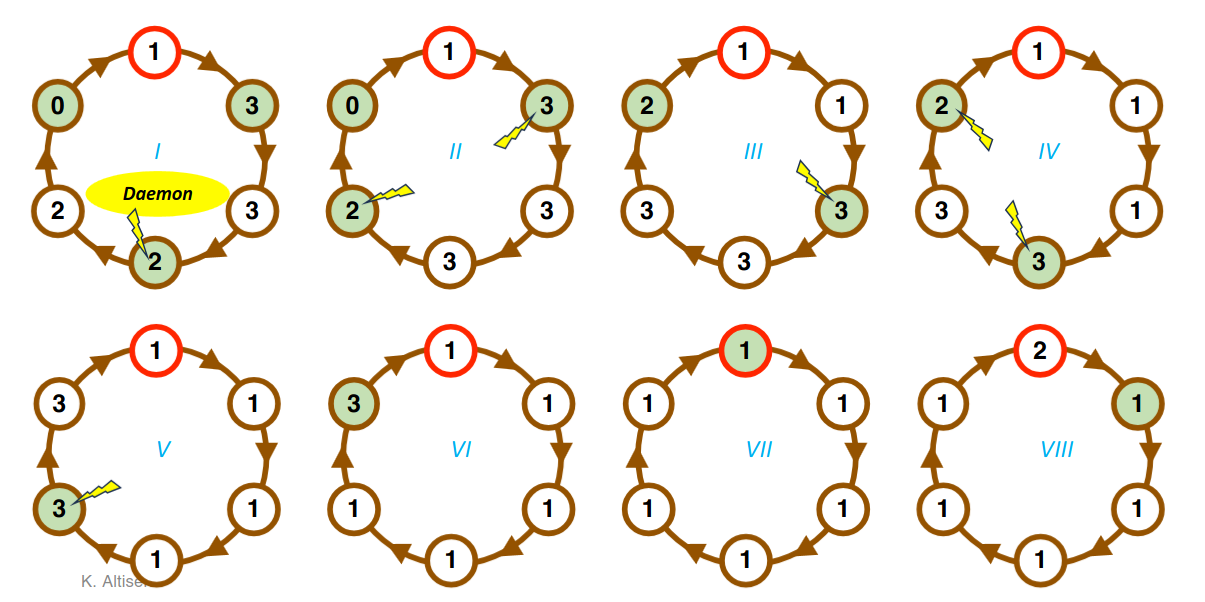
\includegraphics[width=\textwidth]{figs/exec_distribue.png}
    \caption{Exemple d'execution pour un démon distribué}
    \label{fig:ex_disjkstra}
\end{figure}

Les noeuds colorés représentent les noeuds activables et les noeuds avec un éclair correspondent aux noeuds activés.
Pour la première étape, on remarque que trois noeuds sont activables mais seulement un est activé. 
La valeur du noeud activé est alors mis à jour. 
On remarque qu'à partir de l'étape 5, on a atteint un état légitime avec seulement un seul token (un seul noeud activable à chaque tour).

\subsection{Exemple 2 : Coloring}
\label{sec:orgec1e448}

\subsubsection{Algorithme}
\label{sec:orgb184cc9}
L'algorithme de coloration vise à attribuer des couleurs aux nœuds d'un graphe de manière à ce que deux nœuds adjacents n'aient pas la même couleur. 

\begin{enumerate}
\item Chaque nœud \(v\) a un état  \(color(v)\) qui est représenté par un entier positif.
\item Chaque nœud \(v\) observe les couleurs de ses voisins.
\item Si \(v\) détecte qu'il a la même couleur qu'un de ses voisins, il change sa couleur à la première couleur différente des couleurs de ses voisins.
\end{enumerate}

Formellement, l'algorithme peut être écrit comme suit :
\begin{itemize}
\item Garde : \(\exists u \in voisins(v) \, \text{tel que} \, color(v) = color(u)\)
\end{itemize}
où voisins(v) est la liste des voisins du noeud v et color(u) est la couleur du noeud u.
\begin{itemize}
\item Action : \(color(v) \leftarrow \min(\{n \in N* \} \setminus \{color(u) \mid u \in voisins(v)\})\)
\end{itemize}

\subsubsection{Exécution sous démon central}
\label{sec:orgfb5a9a2}
Sous un démon central, à chaque étape, un seul nœud est activé. Voici un exemple simple :

\begin{enumerate}
\item Considérons un graphe avec trois nœuds \(A\), \(B\), et \(C\) formant un anneau.
\item Initialement, \(color(A) = 1\), \(color(B) = 1\), et \(color(C) = 2\).
\end{enumerate}

Le noeud \(A\) et le noeud \(B\) sont activables.
Le démon choisit alors quel noeud sera activé :  

\begin{itemize}
\item \textbf{\textbf{Cas 1 :}} le démon active le noeud \(A\). \(A\) observe que \(B\) a la même couleur (1), donc \(A\) change sa couleur en 3 (première couleur disponible différente de 1 et 2).
\begin{itemize}
\item Nouvelle configuration : \(color(A) = 3\), \(color(B) = 1\), \(color(C) = 2\).
\end{itemize}
\item \textbf{\textbf{Cas 2 :}} Le démon active \(B\). \(B\) observe que \(A\) a la même couleur (1), donc \(B\) change sa couleur en 3 (première couleur disponible différente de 1 et 2).
\begin{itemize}
\item Nouvelle configuration : \(color(A) = 1\), \(color(B) = 3\), \(color(C) = 2\).
\end{itemize}
\end{itemize}

L'algorithme a convergé vers une configuration légitime où tous les nœuds adjacents ont des couleurs différentes.

\subsubsection{Exécution sous démon synchrone}
\label{sec:org2e001c1}
Sous un démon synchrone, tous les nœuds activés changent leur couleur en même temps. Voici un exemple montrant pourquoi cela peut ne pas converger :

\begin{enumerate}
\item Considérons le même graphe initial avec \(color(A) = 1\), \(color(B) = 1\), et \(color(C) = 2\).

\item Le démon synchrone active tous les nœuds enabled.
\begin{itemize}
\item \(A\) et \(B\) observent qu'ils ont la même couleur. \(A\) et \(B\) changent tous les deux leur couleur en 3 (première couleur disponible différente de 1 et 2).
\item Nouvel état : \(color(A) = 3\), \(color(B) = 3\), \(color(C) = 2\).
\end{itemize}
\end{enumerate}

Ainsi, après une étape synchrone, \(A\) et \(B\) ont tout les deux la couleur 3.
On a de nouveaux les noeuds A et B enabled car ils ont tous les deux la couleur 3.
On retrouve la configuration initiale à un rennomage près, ce qui montre que l'algorithme ne converge pas nécessairement vers un état légitime sous un démon synchrone.

\section{Explication des outils}
\label{sec:org445b583}
Pour pouvoir bien comprendre la preuve présente dans why3-do, il est nécessaire de comprendre les outils et les méthodes utilisées.

\subsection{Logique de Hoare}
\label{sec:org2ccc4dc}

\subsubsection{Définition}
\label{sec:org6f96898}
La logique de Hoare est un formalisme utilisé pour raisonner sur la correction des programmes. Elle utilise des triplets de Hoare, notés \{P\} C \{Q\}, où :

\begin{itemize}
\item P est la précondition, une assertion sur l'état des variables du programme avant l'exécution de l'instruction ou du bloc d'instructions C.
\item C est l'instruction ou le bloc d'instructions du programme.
\item Q est la postcondition, une assertion sur l'état des variables du programme après l'exécution de C.
\end{itemize}

Un triplet de Hoare \{P\} C \{Q\} signifie que si la précondition P est vraie avant l'exécution de C, alors la postcondition Q sera vraie après l'exécution de C, à condition que C termine son exécution.

Règles  de la logique de Hoare : 
\begin{enumerate}
\item \textbf{\textbf{Règle de l'assignation}} : Pour une instruction d'assignation x := e,
\begin{itemize}
\item \{P[e/x]\} x := e \{P\}, où P[e/x] est l'assertion P avec toutes les occurrences de x remplacées par e.
\end{itemize}

\item \textbf{\textbf{Règle de composition}} : Pour deux instructions C1 et C2,
\begin{itemize}
\item Si \{P\} C1 \{Q\} et \{Q\} C2 \{R\}, alors \{P\} C1; C2 \{R\}.
\end{itemize}

\item \textbf{\textbf{Règle de la conditionnelle}} : Pour une instruction if (b) then C1 else C2,
\begin{itemize}
\item \{P \(\wedge\) b\} C1 \{Q\} et \{P \(\wedge\) ¬b\} C2 \{Q\} \(\Rightarrow\) \{P\} if (b) then C1 else C2 \{Q\}.
\end{itemize}

\item \textbf{\textbf{Règle de la boucle}} : Pour une boucle while (b) do C,
\begin{itemize}
\item \{I \(\wedge\) b\} C \{I\} \(\Rightarrow\) \{I\} while (b) do C \{I \(\wedge\) ¬b\}, où I est un invariant de boucle.
\end{itemize}
\end{enumerate}


\subsubsection{Exemple}
\label{sec:orgd76cd00}
Considérons la fonction free utilisée dans notre implémentation du coloring dans l'outil why3 en 7.1
Cette fonction renvoie le plus petit entier qui n'est pas présent dans un ensemble :

\lstset{language=why3,label= ,caption= ,captionpos=b,numbers=none}
\begin{lstlisting}
let function free (colors: set) (k:int) : int =
  requires { cardinal colors < k }
  ensures { not mem result colors }
  ensures { forall x. (0 <= x < k /\ not mem x colors) -> result <= x }
  ensures { 0 <= result < k }
  min_elt (diff (interval 0 k) colors)
\end{lstlisting}
Dans le langage de Why3, whyMl, les préconditions sont annotées le mot-clef \texttt{requires} 
et les postconditions par le mot-clef \texttt{ensures}.

Lors de l'appel d'une précondition ou postcondition, l'outil Why3 va générer pour chaque appel de cette fontion, une condition de vérification (VC)
qui sera soumise à un solveur SMT.
\paragraph{Préconditions (requires)}
\label{sec:org7013cf6}


     \texttt{requires \{ cardinal colors < k \}} stipule que la taille (cardinal) 
de l'ensemble \texttt{colors} doit être strictement inférieure à \texttt{k}.
 Cela signifie qu'il existe au moins un entier dans l'intervalle \texttt{[0, k)} qui n'est pas présent dans l'ensemble \texttt{colors}. 
En d'autres termes, l'ensemble \texttt{colors} ne peut pas contenir tous les entiers de 0 à k.

\paragraph{Postconditions (ensures)}
\label{sec:orgd336cf5}


     \texttt{ensures \{ not mem result colors \}}
  Cette postcondition garantit que le résultat (l'entier retourné par la fonction \texttt{free}) ne fait pas partie de l'ensemble \texttt{colors}. 
Autrement dit, \texttt{result} est un entier qui n'est pas présent dans l'ensemble \texttt{colors}.

\texttt{ensures \{ forall x. (0 <= x < k /\textbackslash{} not mem x colors) -> result <= x \}}
  Cette postcondition assure que le résultat est le plus petit entier possible qui n'est pas dans \texttt{colors} et qui se trouve dans l'intervalle [0, k). 
Pour tout entier \texttt{x} dans l'intervalle [0, k) qui n'est pas dans \texttt{colors}, le résultat doit être inférieur ou égal à \texttt{x}. 
Cela garantit que la fonction retourne le plus petit entier manquant.

\texttt{ensures \{ 0 <= result < k \}}
  Cette postcondition garantit que le résultat se situe dans l'intervalle \texttt{[0, k)}. 
Le résultat doit être un entier non négatif et strictement inférieur à \texttt{k}.

\paragraph{Détails de l'implémentation}
\label{sec:org4303a7d}

\texttt{min\_elt (diff (interval 0 k) colors)}
  Cette expression utilise des opérations sur les ensembles pour trouver le résultat.
\begin{itemize}
\item \texttt{interval 0 k} représente l'ensemble des entiers de 0 à k-1.
\item \texttt{diff (interval 0 k) colors} représente l'ensemble des entiers de 0 à k-1 qui ne sont pas dans \texttt{colors}.
\item \texttt{min\_elt} trouve le plus petit élément de cet ensemble, qui est le plus petit entier manquant dans \texttt{colors}.
\end{itemize}

\subsection{SMT solver}
\label{sec:org6cbc25d}

Les SMT (Satisfiability Modulo Theories) solveurs sont des outils puissants utilisés pour 
vérifier la satisfiabilité d'expressions logiques sous certaines contraintes théoriques, 
c'est-à-dire, il vérifie qu'il existe une affectation des variables qui rend la formule vraie, 
en utilisant des théories (comme l'arithmétique, les tableaux, les bit-vectors, etc.).
Les SMT solveurs étendent les capacités des solveurs SAT (Satisfiability), 
qui vérifient la satisfiabilité de formules en logique propositionnelle. 
Alors que les solveurs SAT se concentrent sur des expressions booléennes, 
les SMT solveurs traitent des expressions plus complexes en combinant les solveurs SAT avec des solveurs spécifiques pour diverses théories.
Les formules SMT sont souvent converties en une forme équivalente, que les solveurs SAT peuvent traiter.
Nous allons par la suite utiliser différents solveurs SMT tel que Z3, altErgo et CVC4

\subsection{Why3}
\label{sec:org4f8e959}

Why3 est un outil pour la vérification formelle basé sur la logique de Hoare, 
permettant de garantir leur correction en utilisant des techniques sophistiquées. 
Il permet de spécifier des propriétés formelles à l'aide de contrats, incluant préconditions, postconditions, 
invariants de boucle et variants. 
Ces spécifications sont utilisées pour vérifier que le code respecte les propriétés définies en générant des obligations de preuve que Why3
tente de prouver automatiquement ou manuellement en utilisant la logique de Hoare.

L'IDE de Why3 simplifie le processus de vérification en offrant des outils 
pour visualiser et interagir avec les spécifications et les obligations de preuve. 
Why3 utilise le langage WhyML, basé sur Ml, pour écrire des programmes vérifiables tout en permettant 
l'extraction de code vers OCaml. 
Il peut également collaborer avec divers prouveurs SMT comme AltErgo, Z3 et CVC4, 
ainsi que des assistants de preuve interactifs comme Coq, 
offrant une grande flexibilité pour la vérification formelle.

\section{Why3 do The Way Of Harmonious Distributed System Proofs}
\label{sec:org387140d}

Maintenant nous avons connaissance des différents outils nous pouvons aborder why3-do.
Dans cet article, les auteurs proposent une implémentation d'un modèle instanciable pour des algorithmes
distribués auto-stable ainsi que l'algo du Token Ring de Disjkstra et sa preuve.


Tout d'abord, il est important de comprendre que leur modélisation est séparée en deux parties distinctes. 
La première partie est un modèle instanciable qui est la partie commune aux algorithmes distribués
auto-stabilisants. 
La seconde est propre aux spécifités de l'algorithme et de la topologie dans laquelle celui-ci est appliqué. 


\subsection{Explication du modèle : modelReadallEnabled}
\label{sec:orgb82e974}

Nous commençons par décrire le modèle nommé modelReadallEnabled.
Celui-ci est composé de deux modules Config et Steps.


\subsubsection{Module Config}
\label{sec:orgb493e24}

Dans le module Config (nommé World dans leur papier), on définit les différents types qui seront utilisés dans l'algorithme.
Nous aurons alors le type node, qui représente les noeuds du graphe et le type state qui représente les états que peut prendre un noeud.
On définit alors le type Config comme étant une fonction associant les noeuds à leurs états (map).
Les types node et state ne sont pas définis dans le modèle car ils dépendent de l'algorithme. 
Lorsque l'on décrira l'algorithme il faudra spécifier leurs types, puis instancier le module Config avec ces types à l'aide de mot clé Clone. 

\lstset{language=why3,label= ,caption= ,captionpos=b,numbers=none}
\begin{lstlisting}
module Config
  use int.Int
  use map.Map
  use list.List
  use list.Append
  use list.Mem
  use list.Map as Lmap

  type node
  type state
  type config =  map node state

end

\end{lstlisting}

\subsubsection{Module Steps}
\label{sec:org3dadd0e}

Le second module est une formalisation en whyml du modèle atomique à état.
De la même manière que Config c'est un modèle à instancier,
on retrouve les types node et state et différentes fonctions ou prédicats à instancier grâce au mot-clef \texttt{val}. 
Le prédicat validNd indique si un noeud n est valide; ce prédicat permet de mettre des conditions sur les noeuds 
\texttt{case\_node} et \texttt{case\_state} assurent que le résultat est toujours vrai pour un noeud/état donné.
\lstset{language=why3,label= ,caption= ,captionpos=b,numbers=none}
\begin{lstlisting}

module Steps
  use int.Int
  use map.Map
  use list.List
  use list.Mem
  use list.Append
  use list.Map as Lmap


  type node
  type state
  type config = map node state

  val predicate validNd (n:node)

  val predicate case_node (node)
    ensures { result }

  val predicate case_state (state)
    ensures { result }

\end{lstlisting}

On remarque un premier problème dans le modèle de why3-do qui est que l'état initial est fixé et 
doit être instancié, ce qui est une limitation très restrictive pour un algorithme distribué auto-stable;
on voudrait pouvoir faire des preuves pour toutes configuartions initiales.

Dans le code whyml ci-dessous \texttt{indpred} est un prédicat inductif qui va faire office d'invariant dans la preuve des programmes instanciés, 
de plus ce prédicat doit être vrai pour la configuration initiale. 

On remarque l'utilisation du mot-clef \texttt{ghost}. Cette notation indique que le prédicat ici est seulement présent dans 
les spécifications et non dans le code exécutable. Cela permet d'ajouter des informations pour faciliter la
preuve de programme.
\lstset{language=why3,label= ,caption= ,captionpos=b,numbers=none}
\begin{lstlisting}


val function initState (node) : state

constant initConfig : config = initState

val ghost predicate indpred (c : config)
  ensures { c=initConfig -> result }

\end{lstlisting}
Le prédicat \texttt{enabled} est la condition pour laquelle le noeud est activable.

\texttt{let ghost function step\_enbld (c: config) (n: node) (s: state): config} : met à jour la configuration \texttt{c} en remplaçant l'état du nœud \texttt{n} par \texttt{s}.
handleEnbld est une fonction qui gère un nœud activé dans une configuration, c'est la fonction qui va choisir la nouvelle valeur de l'état pour un noeud
en s'assurant la préservation du prédicat inductif après la mise à jour. 
\lstset{language=why3,label= ,caption= ,captionpos=b,numbers=none}
\begin{lstlisting}

val ghost predicate enabled (config) (n:node)
  requires { validNd n }

let ghost function step_enbld (c:config) (n:node) (s:state) : config =
  set c n s

val function handleEnbld (n:node) (c : config) : state
  requires { validNd n }
  requires { enabled c n}
  requires { indpred c }
  requires { case_node n }
  ensures  { indpred (step_enbld c n result) }

\end{lstlisting}

\texttt{step} est un invariant inductif qui décrit une transition d'une configuration à une autre après l'activation d'un noeud.
La ligne \texttt{step c n (step\_enbld c n (handleEnbld n c))} signifie que l'on passe de la configuration \texttt{c} à la configuration dans laquelle le noeud \texttt{n} a été mise à jour. 
Cela implique qu'il n'y a qu'un seul noeud qui peut être activé au même moment, donc cela fixe le démon comme un démon central. 

\lstset{language=why3,label= ,caption= ,captionpos=b,numbers=none}
\begin{lstlisting}

inductive step config node config =
| step_enbld : forall c: config , n :node.
    validNd n ->
      enabled c n ->
	step c n (step_enbld c n (handleEnbld n c))

\end{lstlisting}
Le lemme \texttt{indpred\_step} assure que le prédicat \texttt{inductive} est conservé après un \texttt{step} ce qui est facilement prouvable grâce aux postconditions de \texttt{handleEnbld}.
Le lemme \texttt{step\_preserves\_states} assure que lorsque un noeud est modifié alors tout les autres n'ont pas changé. 
\texttt{step\_TR} est la fermeture transitive de \texttt{step} : 
\begin{itemize}
\item Cas de base : Pour toute configuration \texttt{c} peut s'atteindre elle-même en 0 étape.
\item Cas inductif : Pour toute configuration \texttt{c}, \texttt{c'}, et \texttt{c''} il existe une séquence de steps pour aller de \texttt{c} à \texttt{c'} et il existe une transition unique pour aller de \texttt{c'} à \texttt{c''} via le noeud \texttt{n}.
\end{itemize}
\lstset{language=why3,label= ,caption= ,captionpos=b,numbers=none}
\begin{lstlisting}

lemma indpred_step :
  forall c c' :config, n :node. step c n c' -> indpred c -> indpred c'

lemma step_preserves_states :
  forall c c' :config, n1 n2 :node. step c n1 c' -> n2<>n1 -> c n2 = c' n2


inductive step_TR config config int =
| base : forall c: config. step_TR c c 0
| step : forall c c' c'' :config, n :node, steps :int.
  step_TR c c' steps -> step c' n c'' -> step_TR c c'' (steps+1)

\end{lstlisting}
Le lemme \texttt{noNegative\_step\_TR} assure que le nombre de steps pour passer d'une configuration à une autre est toujours positif.
Le prédicat \texttt{reachable} vaut vrai s'il existe un nombre d'étapes pour atteindre la configuration c depuis la configuration initiale.
\texttt{indpred\_manySteps} assure que le prédicat inductif est conservé par plusieurs étapes.
\texttt{indpred\_reachable} étend le lemme précédent à l'aide de reachable en assurant que le prédicat inductif reste vrai pour toutes les configurations atteignables. 
\lstset{language=why3,label= ,caption= ,captionpos=b,numbers=none}
\begin{lstlisting}

lemma noNegative_step_TR : forall c c': config, steps :int.
  step_TR c c' steps -> steps >= 0

predicate reachable (c:config) = exists steps :int. step_TR initConfig c steps

lemma indpred_manySteps :
  forall c c' :config, steps :int . step_TR c c' steps -> indpred c -> indpred c'

lemma indpred_reachable :
  forall c: config. reachable c -> indpred c

\end{lstlisting}


\subsection{Explication de selfstab-ring}
\label{sec:org6b923a9}
Nous allons faire une explication rapide de la preuve de l'algorithme de Token Ring de Dijkstra.

La preuve est séparée en deux parties, la cloture : depuis un état légitime, on reste dans un état légitime 
puis la terminaison : à partir d'un état non légitime, en un nombre fini d'étape, on atteint un état légitime.

\subsubsection{Cloture}
\label{sec:org3d8eb84}
Pour définir l'algorithme, ils vont implémenter les différents types, prédicats et fonctions du modèle à instancier, c'est à dire à chaque fois
qu'il y avait le mot-clef \texttt{val}.


Dans un premier temps ils choisissent de définir les noeuds et les états comme des entiers. 
Ils peuvent alors définir le type \texttt{config} en clonant le module \texttt{Config} du modèle. 


\lstset{language=why3,label= ,caption= ,captionpos=b,numbers=none}
\begin{lstlisting}

type node = int
type state = int


clone modelReadallEnabled.Config with
  type node,
  type state,

\end{lstlisting}



Puis ils définissent un noeud valide comme un entier compris entre \texttt{0} et \texttt{n\_nodes}.
Puis définissent \texttt{has\_token}, \texttt{atMostOneToken} et \texttt{atLeastOneToken} qui permettent de définir l'invariant \texttt{indpred}.
L'invariant est alors : les noeuds sont entre 0 et une borne max, et les état sont entre 0 et une borne max et il y a au moins token.
On note également que l'état initial choisi est la racine vaut 1 et les autres noeuds valent 0.
L'état initial est donc bien légitime.

Puis ils définissent différentes fonctions et prédicats pour pouvoir instancier leur modèle.

Une fois que tout est définit, il suffit d'utiliser de prouver que tout état atteignable depuis l'état initial prouve \texttt{oneToken}.

\lstset{language=why3,label= ,caption= ,captionpos=b,numbers=none}
\begin{lstlisting}

  val constant n_nodes : int
  let predicate validNd (n:node) = 0 <= n < n_nodes



  let predicate case_node (_node) = true
  let predicate case_state (_state) = true

  let function incre (x:state) : state
  = mod (x+1) k_states


  let function initState (n:node) : state
  = if n=n_nodes-1 then 1 else 0

  predicate has_token (c:config) (n:node) =
  (n = 0 /\  c n =  c (n_nodes-1))
  \/
  (n > 0 /\ n < n_nodes /\ c n <> c (n-1))

  let ghost predicate enabled (c : config) (n:node)
  = has_token c n

  let function handleEnbld (n:node) (c:config) : state
  = if n = 0 then incre (c (n_nodes-1))
	     else c (n-1)

  predicate inv (c:config) =
    (forall n :int. 0 <= n < n_nodes -> 0 <= c n < k_states)
    /\
    atMostOneToken c n_nodes

  let ghost predicate indpred (c:config) = inv (c)


  (* Cloning the Steps module will generate VCs to ensure that indpred is an inductive invariant *)
  clone modelReadallEnabled.Steps with
    type node,
    type state,
    val validNd,
    val case_node,
    val case_state,
    val initState,
    val indpred,
    val enabled,
    val handleEnbld


  predicate oneToken (w:world) = atMostOneToken w n_nodes /\ atLeastOneToken w n_nodes

  goal oneToken : forall w :world. reachable w -> oneToken w

end



\end{lstlisting}
\subsubsection{Terminaison}
\label{sec:org5f73062}

Dans la seconde partie le modèle est réinstancié avec des valeurs initiales différentes 
L'état initial n'est plus un état légitime et on cherche à atteindre l'état \texttt{converged} qui 
est défini comme tous les noeuds qui ont la même valeur. Cet état est un état légitime. 

\lstset{language=why3,label= ,caption= ,captionpos=b,numbers=none}
\begin{lstlisting}
predicate initConv (c:config) =
  exists j : int. 0<=j<n_nodes /\ (forall k :int. 0<k<=j -> c k = c 0) /\ noOcc_from c (c 0) (j+1)

predicate converged (c:config) =
  forall n :node. validNd n -> c n = c 0

\end{lstlisting}


Pour prouver qu'en partant d'un état initial, on arrive bien à cet état légitime, 
la méthode proposée est d'utiliser une fonction de potentiel \texttt{measureAllNodes},
une fonction récursive qui somme le potentiel de chaque noeud.



On associe une valeur entière positive au graphe en fonction de ses états.
On montre que lorsque l'on atteint converged alors la mesure vaut 0. 
Et que cette mesure décroit bien d'au moins 1 à chaque step. 


\lstset{language=why3,label= ,caption= ,captionpos=b,numbers=none}
\begin{lstlisting}

let ghost function measureAllNodes (w:world) : int
  requires { indpred w }
  ensures  { result >= 0 }
  (* ensures  { result = 0 -> converged w } *)
  ensures  { not (converged w) -> result > 0 }   (* equivalent to the previous formulation *)
= measureNodes w n_nodes

\end{lstlisting}

Pour faire cela, Why3do détaille cas par cas les différentes exécutions possibles comme nous
pouvons le voir dans les nombreux ensures de \texttt{measureDeltaNodes}. 
Cela permet à Why3 de prouver \texttt{step\_decresasesMeasure} (la mesure de la configuration décroit lorsque l'on fait un step)
 et \texttt{converged\_oneToken} (lorsque la mesure vaut 0, alors il y a un seul token et il se trouve à la racine).  

\lstset{language=why3,label= ,caption= ,captionpos=b,numbers=none}
\begin{lstlisting}

let rec ghost function measureDeltaNodes (w:world) (w':world) (n:int) (k:node) : int
  requires { indpred w }
  requires { 1 <= n <= n_nodes }
  requires { validNd k }
  requires { step w k w' }
  ensures  { result = measureNodes w' n - measureNodes w n }
  ensures  { 0 <= n-1 < k -> result + n_nodes * mod (convState w - convState w') k_states = 0 }
  ensures  { n>1 -> k = n-1 -> result + n_nodes * mod (convState w - convState w') k_states = n-1-n_nodes }
  ensures  { n>0 -> k = 0 -> convState w' <> convState w -> result + n_nodes * (diffZero w (convState w)) <= 0 }
  ensures  { n>0 -> k = 0 -> convState w' =  convState w -> result < 0 }
  ensures  { 0 <= k < n-1 -> result < 0 }
  ensures  { n = n_nodes -> result < 0 }
  variant  { n }
= if n=1 then measureDeltaNode w w' 0 k
  else measureDeltaNode w w' (n-1) k + measureDeltaNodes w w' (n-1) k

goal step_decreasesMeasure : forall w w' :world, k :node.
  indpred w -> step w k w' -> measureAllNodes w' < measureAllNodes w


goal converged_oneToken : forall w :world. converged w -> oneToken w /\ has_token w 0

\end{lstlisting}

\section{Implémentation et preuve de l’algorithme de coloring basé sur le modèle de why3-do}
\label{sec:orgd994304}

Nous allons maintenant montrer comment j'ai implémenté et prouvé l'algorithme de coloration en nous basant sur le modèle proposé par why3-do.
Nous allons suivre les méthodes présentées dans le chapitre précédent pour cette implémentation.

\subsection{Cloture}
\label{sec:org7e1a303}

Pour la cloture, notre objectif est d'instancier le modèle. 

Pour cela, nous créons un nouveau module et nous importons les différentes bibliothèques dont nous aurons besoin. 
\begin{itemize}
\item Les listes
\item Les entiers
\item La division euclidienne pour pouvoir faire des modulos
\item Les maps (associations de valeurs d'un type à un autre)
\item Les ensembles d'entiers
\end{itemize}

\lstset{language=why3,label= ,caption= ,captionpos=b,numbers=none}
\begin{lstlisting}

module Coloring_Ring
 use list.List
 use int.Int
 use int.EuclideanDivision
 use map.Map
 use list.Mem
 use set.SetAppInt

\end{lstlisting}

Dans un premier temps, on souhaite montrer la cloture.
Pour cela, on commence à définir les objets et règles avec lesquels on veut travailler. 
On définit \texttt{n\_nodes}, une constante entière qui représente le nombre de noeud de notre système. 
De la même manière on définit \texttt{k\_color} qui représente le nombre de couleurs disponibles.

Nous nous plaçons dans un anneau, il nous faut au minimum 3 noeuds. 
Il faut s'assurer que le graphe soit coloriable, pour cela il suffit de s'assurer qu'il y a plus de couleurs disponibles que de noeuds, c'est à dire au moins une couleur par noeud. 
Pour cela on utilise le mot clé \texttt{axiom}, il faut être très délicat avec ce mot clé car il est facile d'écrire une contradiction. 

\lstset{language=why3,label= ,caption= ,captionpos=b,numbers=none}
\begin{lstlisting}

val constant n_nodes : int

axiom at_least_three : 2 < n_nodes

val constant k_color : int

axiom k_color_bound : n_nodes <= k_color

\end{lstlisting}
Puis on définit les types que l'on va utiliser. 
On choisit de représenter les noeuds par des entiers.
Pour l'état du noeud (sa couleur) on utilise une structure contenant un entier.
On définit alors le type \texttt{config} comme étant le map entre les noeuds et les états.


\lstset{language=why3,label= ,caption= ,captionpos=b,numbers=none}
\begin{lstlisting}

type node = int

type state = {k: int}

clone modelReadallEnabled.Config with
  type node,
  type state


\end{lstlisting}
Ici nous ajoutons le prédicat qui signifie qu'un noeud est valide s'il est compris entre \texttt{0} et \texttt{n\_nodes} le nombre de noeuds
\lstset{language=why3,label= ,caption= ,captionpos=b,numbers=none}
\begin{lstlisting}

let predicate validNd (n:node) = 0 <= n < n_nodes

\end{lstlisting}

Le prédicat is\_neighbor vérifie si deux nœuds i et j sont voisins dans un anneau de nœuds, on préfère détailler chaque cas pour ne pas utiliser
l'arithmétique modulaire qui peut poser problème pour les prouveurs SMT.

\lstset{language=why3,label= ,caption= ,captionpos=b,numbers=none}
\begin{lstlisting}

predicate is_neighbor (i : int) (j : int) =
  validNd i -> validNd j ->
   if i = 0         then j=1 \/ j=n_nodes-1 else
   if i = n_nodes-1 then j=0 \/ j=n_nodes-2 else
   j = i-1 \/ j = i+1

predicate is_neighbor_in_a_ring (i:int) (j:int) = is_neighbor i j

\end{lstlisting}


Le lemme \texttt{is\_neigbhor\_symetric} affirme que le prédicat \texttt{is\_neighbor} est symétrique. En d'autres termes, si i est un voisin de j, alors j est aussi un voisin de i.
\texttt{not\_its\_own\_neighbor} stipule qu'aucun nœud n'est son propre voisin. Si i est un nœud valide, il ne peut pas être voisin de lui-même.
Ces deux lemmes sont nécessaires pour prouver les clauses de la prochaine fonction \texttt{neighbor\_set}. 

\lstset{language=why3,label= ,caption= ,captionpos=b,numbers=none}
\begin{lstlisting}

lemma is_neighbor_symmetric: forall i j. is_neighbor i j = is_neighbor j i

lemma not_its_own_neighbor : forall i.  validNd i -> not (is_neighbor i i)


\end{lstlisting}

La fonction \texttt{neighbor\_set} prend un nœud i en entrée et retourne l'ensemble de ses voisins.

Les voisins du nœud i sont calculés de la manière suivante :
    next est le nœud immédiatement après i, calculé comme \texttt{(i+1) mod n\_nodes}.
    prev est le nœud immédiatement avant i, calculé comme \texttt{(i-1) mod n\_nodes}.
L'ensemble des voisins est ensuite créé en ajoutant \texttt{next} et prev\textasciitilde{} à un ensemble vide.

Clauses \texttt{ensures} (Conditions que la fonction garantit après son exécution) :

Les deux premières clauses : Les nœuds prev et next sont bien des voisins de i.

Clause suivante : Aucun nœud n'est son propre voisin (c'est-à-dire que i n'est pas dans le résultat).

Clause de cardinalité : L'ensemble des voisins a exactement 2 éléments, ce qui est spécifique à la structure en anneau où chaque nœud a exactement deux voisins.

Clause de validité : Tous les nœuds dans l'ensemble résultant sont des nœuds valides.

Clauses de voisinage : Chaque nœud dans l'ensemble résultant est un voisin de i, et chaque voisin valide de i est dans l'ensemble résultant.

\lstset{language=why3,label= ,caption= ,captionpos=b,numbers=none}
\begin{lstlisting}

let function neighbor_set (i:node): set
  requires { validNd i }

  ensures { is_neighbor (mod (i-1) n_nodes) i } 
  ensures { is_neighbor (mod (i+1) n_nodes) i } 
  ensures { forall c. mem c result -> c <> i} 
  ensures {  cardinal result = 2 } 
  ensures { forall j. mem j result -> validNd j }
  ensures { forall j. mem j result -> is_neighbor  i j }
  ensures { forall j. validNd j -> is_neighbor i j -> mem j result }
  =
  let next = mod (i+1) n_nodes in
  let prev = mod (i-1) n_nodes in
  add next (add prev (empty()))


\end{lstlisting}

La fonction \texttt{free} prend en entrée un ensemble \texttt{colors} de valeurs entières et un entier \texttt{k}. 
Elle retourne la plus petite valeur entière qui n'est pas présente dans l'ensemble colors et qui se trouve dans l'interval \texttt{[0, k-1]}.

\lstset{language=why3,label= ,caption= ,captionpos=b,numbers=none}
\begin{lstlisting}
let function free (colors: set) (k:int) : int =
  requires { cardinal colors < k }
  ensures { not mem result colors }
  ensures { forall x. (0 <= x < k /\ not mem x colors) -> result <= x }
  ensures { 0 <= result < k }
  min_elt (diff (interval 0 k) colors)


\end{lstlisting}

Nous devons une fois de plus choisir la valeur initial des états, il semble cohérent de les fixer tous à 0, la plus petite valeur possible.

\lstset{language=why3,label= ,caption= ,captionpos=b,numbers=none}
\begin{lstlisting}

  let function initState (n:node) : state =
  {k=0}

let function color (c:config) (n:node)  : int =
   (c n).k

\end{lstlisting}

La fonction \texttt{get\_colors} récupère les couleurs associées à un ensemble d'éléments \texttt{nl} à partir d'une configuration c. 
La postcondition \texttt{ensures \{ forall coul. mem coul result <-> exists x. mem x nl /\textbackslash{} coul = (c x).k \}} signifie
que pour chaque couleur \texttt{coul}, \texttt{coul} est un élément du résultat (\texttt{result}) si et seulement si 
il existe un élément \texttt{x} dans l'ensemble \texttt{nl} tel que \texttt{coul} est la couleur associée à \texttt{x} dans la configuration \texttt{c}.
Cette postcondition est nécessaire pour prouver la suite du programme.

\lstset{language=why3,label= ,caption= ,captionpos=b,numbers=none}
\begin{lstlisting}

let rec function get_colors (nl:set) (c:config) : set =
   requires { cardinal nl < 3 }
   ensures { cardinal result <= cardinal nl }
   ensures { forall coul. mem coul result <-> exists x. mem x nl /\ coul = (c x).k }
   variant { cardinal nl }
   if is_empty nl then empty () else
    let n = choose nl in
    let coul = color c n in
    add coul (get_colors (remove n nl) c)


\end{lstlisting}

Le prédicat \texttt{conflict} est défini tel que pour un noeud, on regarde ses voisins et on vérifie s'il en existe un qui a la même couleur.

\lstset{language=why3,label= ,caption= ,captionpos=b,numbers=none}
\begin{lstlisting}

predicate conflict (c: config) (n:node) =
   exists coul : int.
     mem coul (get_colors (neighbor_set n) c) /\ (c n).k = coul



\end{lstlisting}

On instancie notre modèle en spécifiant qu'un noeud est activalbe quand il a un conflit (au moins un voisin ayant la même couleur que lui).
Et la fonction de calcul de la nouvelle couleur (\texttt{handleEnbld}), sera un appel à \texttt{free}. 
Ici \texttt{k} est la couleur de l'état (par rapport à l'invariant de définition)

\lstset{language=why3,label= ,caption= ,captionpos=b,numbers=none}
\begin{lstlisting}

let predicate enabled (c:config) (n:node)
   ensures { validNd n -> result = conflict c n }
   =  validNd n &&  mem (c n).k (get_colors (neighbor_set n) c)


  let function handleEnbld (n:node) (c:config) : state
    requires { validNd n }
    ensures { not mem result.k (get_colors (neighbor_set n) c) }
    ensures { forall i. mem i (neighbor_set n) -> not conflict c i -> not conflict (set c n result) i }
    =
    { k = free (get_colors (neighbor_set n) c) k_color }

\end{lstlisting}

Dans notre invariant nous voulons garantir que que les états des noeuds sont valides et donc le reste durant l'exécution du programme.
Nous pouvons alors instancier/cloner \texttt{modelReadallEnabled}

\lstset{language=why3,label= ,caption= ,captionpos=b,numbers=none}
\begin{lstlisting}


predicate inv (c: config) =
  (forall n: node. 0 <= n < n_nodes -> 0 <= (c n).k <= k_color)

let ghost predicate indpred (c:config) = inv c


clone modelReadallEnabled.Steps with
    type node, type state, val validNd, val indpred, val enabled, val handleEnbld, val initState



\end{lstlisting}

On définit alors le prédicat \texttt{colored} qui vérifie que tout les noeuds sont bien coloriés, 
puis \texttt{no\_conflict}, un prédicat qui renvoie true si pour tout les noeuds il n'y a pas de conflits.
On peut alors écrire notre goal : \texttt{goal\_colored} qui spécifie que pour tout état atteignable (depuis 
la configuration initiale) s'il n'y a pas de conflit pour la configuration alors le configuration 
est bien coloriée. 

\lstset{language=why3,label= ,caption= ,captionpos=b,numbers=none}
\begin{lstlisting}

predicate colored (c:config) =
  forall n1: node.
    validNd n1 ->
    couleurDifferentes c n1

predicate no_conflict (c: config) = forall n: node. not(conflict c n)

goal goal_colored : forall c:config. reachable c -> no_conflict c -> colored c

end

\end{lstlisting}

\subsection{Terminaison}
\label{sec:org637ad0f}

Nous allons maintenant montrer la terminaison de l'algorithme. 
Pour cela, nous allons utiliser une fonction de potentiel. 
Cette fonction permettra d'évaluer la valeur d'une configuration.


Nous commençons alors par définir le potentiel d'un noeud comme étant 1 s'il y a un conflit, 
c'est à dire un noeud de la même couleur parmi ses voisins. 

\lstset{language=why3,label= ,caption= ,captionpos=b,numbers=none}
\begin{lstlisting}

let ghost function potential_node (c:config) (n:int) : int
  ensures { 0 <= result <= 1 }
  ensures { result = 1 <-> conflict c n }
  =
  if conflict c n then 1 else 0


\end{lstlisting}
Puis nous définissons la fonction de potentiel sur la configuration entière en faisant la somme
de tout ses noeuds. 

La fonction récursive \texttt{potential\_i} calcule le potentiel de conflit pour les \texttt{i} premiers nœuds d'une configuration donnée \texttt{c}. 
Elle prend en entrée cette configuration ainsi qu'un entier \texttt{i}, représentant un index de nœud. 

La clause \texttt{requires} garantit que l'index \texttt{i} correspond bien à un nœud valide. 
Le résultat renvoyé par la fonction est toujours non négatif. 
Si tous les nœuds de \texttt{0} à \texttt{i} ne présentent aucun conflit (c'est-à-dire que la fonction \texttt{potential\_node c j} renvoie 0 pour chaque \texttt{j} dans cet interval), 
alors le résultat sera 0 ; sinon, il sera strictement supérieur à 0. 

La fonction commence par calculer le potentiel de conflit pour le nœud \texttt{i} actuel (\texttt{pot\_i}), 
puis ajoute ce potentiel à celui des nœuds précédents de manière récursive. 

La clause \texttt{variant \{ i \}} assure que la récursion terminera correctement, 
car l'index \texttt{i} diminue à chaque appel récursif.

La fonction potential est juste un appel de \texttt{potential\_i} pour tous les noeuds, en gardant les mêmes clauses.

\lstset{language=why3,label= ,caption= ,captionpos=b,numbers=none}
\begin{lstlisting}


let rec ghost function potential_i (c:config) (i:int) : int
    requires { validNd i }
    ensures  { result >= 0 }
    ensures  { result = 0 <-> forall j :int. 0<=j<=i -> potential_node c j = 0 }
    variant  { i }
  =
	let pot_i = if conflict c i then 1 else 0 in
	if i=0 then pot_i
	       else pot_i + potential_i c (i-1)


let ghost function potential (c:config) : int
    ensures  { result >= 0 }
    ensures  {  exists n:node. conflict c n -> (potential_node c n = 1) -> (result> 0)}
    ensures  { result = 0 <-> forall i :int. 0 <= i < n_nodes -> potential_node c i = 0 }

  = potential_i c (n_nodes-1)


\end{lstlisting}
Nous pouvons maintenant écrire quelques lemmes qui seront nécessaire pour faire les preuves suivantes. 

\begin{itemize}
\item \texttt{step\_on\_n\_preserves\_other\_nodes} affirme que lorsqu'une étape de transformation (\texttt{step}) est effectuée sur un nœud \texttt{n} dans la configuration \texttt{c},
\end{itemize}
la valeur de tous les autres nœuds (\texttt{i}) reste inchangée dans la nouvelle configuration \texttt{c'} si \texttt{i} n'est pas égal à \texttt{n}.

\begin{itemize}
\item \texttt{no\_conflict\_after\_step} affirme que si une étape de transformation (\texttt{step}) est effectuée sur un nœud \texttt{k} dans la configuration \texttt{c},
\end{itemize}
alors le nœud \texttt{k} ne sera plus en conflit dans la nouvelle configuration \texttt{c'}.

\begin{itemize}
\item \texttt{step\_influences\_neighborhood\_only} affirme que lorsqu'une étape de transformation (\texttt{step}) est effectuée sur un nœud \texttt{n} dans la configuration \texttt{c},
\end{itemize}
seuls les nœuds voisins ou le nœud lui-même peuvent voir leur valeur modifiée dans la nouvelle configuration \texttt{c'}, tandis que tous les autres nœuds restent 
\lstset{language=why3,label= ,caption= ,captionpos=b,numbers=none}
\begin{lstlisting}

lemma step_on_n_preserves_other_nodes :
    forall c c' :config, n i :node. step c n c' -> i<>n -> c i = c' i


lemma no_conflict_after_step: forall c, c', k. step c k c' -> not(conflict c' k)

lemma step_influences_neighborhood_only: forall c c' n i.
  step c n c' ->
     not is_neighbor i n /\ i <> n -> c i = c' i

\end{lstlisting}


Nous voulons maintenant montrer que cette fonction de potentiel décroît à chaque fois qu'un nœud est activé. Pour cela, nous définissons la fonction \texttt{deltaPotAfterStep\_i}.

Explication :

\begin{itemize}
\item Cette fonction récursive calcule la différence de potentiel de conflit entre deux configurations, \texttt{c} et \texttt{c'},
\end{itemize}
pour les \texttt{i} premiers nœuds après l'application d'une étape de transformation (\texttt{step}) sur un nœud spécifique \texttt{n}.

\begin{itemize}
\item Paramètres :
\begin{itemize}
\item \texttt{c} et \texttt{c'} : Les configurations avant et après l'étape de transformation.
\item \texttt{i} : L'index du nœud jusqu'auquel on calcule la variation de potentiel.
\item \texttt{n} : Le nœud sur lequel la transformation (\texttt{step}) a été appliquée.
\item \texttt{pos} : Un booléen indiquant si l'index \texttt{i} a déjà atteint ou dépassé le nœud \texttt{n}.
\item \texttt{delta} : La somme partielle de la variation de potentiel accumulée jusqu'à \texttt{i}.
\end{itemize}

\item Corps de la fonction :
\begin{itemize}
\item La fonction commence par calculer la différence de potentiel pour le nœud \texttt{i} (c'est-à-dire la différence entre \texttt{potential\_node c i} et \texttt{potential\_node c' i}).
\item Si \texttt{i} est égal à 0, la fonction retourne cette différence.
\item Sinon, la fonction additionne cette différence à celle des nœuds précédents (calculée récursivement en appelant \texttt{deltaPotAfterStep\_i} avec \texttt{i-1}).
\end{itemize}

\item Clauses ensures :
\begin{itemize}
\item Si \texttt{i} est égal à \texttt{n}, la différence doit être positive.
\item Si \texttt{pos} est faux (c'est-à-dire si \texttt{i} n'a pas encore atteint \texttt{n}), la différence doit être positive.
\item Le résultat est non négatif et correspond à la différence de potentiel pour les \texttt{i} premiers nœuds entre \texttt{c} et \texttt{c'}.
\end{itemize}
\end{itemize}

La fonction \texttt{deltaPotAfterStep} est un appel à \texttt{deltaPotAfterStep\_i} pour calculer la différence de potentiel pour tous les nœuds d'une configuration.


\lstset{language=why3,label= ,caption= ,captionpos=b,numbers=none}
\begin{lstlisting}

let rec ghost function deltaPotAfterStep_i (c:config) (c':config) (i:int) (n:node) (pos : bool) (delta:int) : int
    requires { validNd i }
    requires { validNd n }
    requires { step c n c' }
    requires { pos <-> exists j. i<j<n_nodes /\ j = n }

    ensures { i = n -> result > 0 }
    ensures  { not pos -> result > 0 }
    ensures  { result >= 0 }
    ensures  { result = potential_i c i - potential_i c' i  }
    variant  { i }
  =
    let delta_i_n = potential_node c i - potential_node c' i in
    if i = 0 then delta_i_n
	     else delta_i_n + deltaPotAfterStep_i c c' (i-1) n (pos || i=n ) (delta+delta_i_n)

let ghost function deltaPotAfterStep (c:config) (c':config) (k:node) : int
   requires { validNd k }
   requires { step c k c' }
    ensures { result > 0 }
    ensures { result = potential c - potential c'}
  = deltaPotAfterStep_i c c' (n_nodes-1) k false 0

\end{lstlisting}


\begin{itemize}
\item \texttt{the\_potential\_decreases\_after\_a\_step} affirme que si une étape de transformation (\texttt{step}) est effectuée sur un nœud valide \texttt{n}
\end{itemize}
dans une configuration \texttt{c}, alors le potentiel total de conflit de la configuration \texttt{c'} après la transformation sera strictement inférieur à celui de la configuration initiale \texttt{c}.

\begin{itemize}
\item \texttt{config\_potential\_is\_null\_iff\_all\_states\_one\_are\_null} établit une équivalence entre le potentiel total d'une configuration et les potentiels de chaque nœud.
\end{itemize}
Il affirme que le potentiel total d'une configuration \texttt{c} est nul si et seulement si tous les nœuds ont un potentiel nul (c'est-à-dire qu'aucun nœud n'est en conflit).


\lstset{language=why3,label= ,caption= ,captionpos=b,numbers=none}
\begin{lstlisting}

lemma the_potential_decreases_after_a_step : forall c c' : config, n :node.
  validNd n -> step c n c' -> potential c > potential c'

lemma config_potential_is_null_iff_all_states_one_are_null :
  forall c : config. (potential c = 0) <-> (forall n: node. 0 <= n < n_nodes -> potential_node  c n = 0)

\end{lstlisting}


Il ne reste plus qu'à créer les prédicats \texttt{no\_conflict} et \texttt{colored} pour pouvoir écrire nos 'goal'.

\begin{itemize}
\item \texttt{no\_conflict} indique qu'il n'y a aucun conflit dans la configuration \texttt{c}.

\item \texttt{colored} indique que la configuration \texttt{c} est correctement colorée, ce qui signifie que tous les nœuds valides n'ont aucun conflit.
\end{itemize}


\lstset{language=why3,label= ,caption= ,captionpos=b,numbers=none}
\begin{lstlisting}

predicate no_conflict (c: config) = forall n: node. not(conflict c n)

predicate colored (c: config) =
  forall n: node.
    validNd n -> not conflict c n

\end{lstlisting}


\texttt{goal\_colored} affirme que pour toute configuration \texttt{c} atteignable à partir d'une configuration initiale \texttt{c\_init}, 
si \texttt{c} n'a aucun conflit (\texttt{no\_conflict c}), alors \texttt{c} est correctement colorée (\texttt{colored c}).

\texttt{goal\_converged} affirme que pour toute configuration \texttt{c}, le potentiel de \texttt{c} est nul si et seulement si \texttt{c} est correctement colorée.


\lstset{language=why3,label= ,caption= ,captionpos=b,numbers=none}
\begin{lstlisting}

goal goal_colored : forall c, c_init :config. reachable c -> no_conflict c -> colored c

goal goal_converged : forall c : config. (potential c = 0) <-> colored c

\end{lstlisting}


Nous avons alors la convergence puisque nous avons prouvé que la fonction de potentiel est positive, 
elle décroît à chaque \texttt{step}, et quand elle est nulle, nous avons atteint la configuration voulue.




\subsection{Quelques remarques}
\label{sec:org9361e43}
\subsubsection{Différents solveurs SMT}
\label{sec:org71b1b60}
Nous observons que d'avoir différents solveurs SMT peut être très avantageux, la plupart des solveurs n'arrivent pas à prouver
La fonction \texttt{free} définit en 7.1 là où CVC5 met moins de 3 secondes.

\subsubsection{Topologie}
\label{sec:org4acdc9f}

Pour essayer de limiter l'impact de la topologie dans l'algorithme nous n'avons que 
neighbor\_set qui dépends de la topologie en anneau,
alors que dans leur implémentation du token ring, celle-ci était présente à de nombreux endroits
\subsection{Problèmes rencontrés}
\label{sec:org02bdcd8}

Lors de la mise en œuvre du programme, plusieurs défis importants ont été identifiés. 
Tout d'abord, la présence implicite d'axiomes faux au début du programme a entraîné des erreurs significatives, 
soulignant l'importance cruciale d'exécuter le détecteur de dysfonctionnements ("smoke detector") en amont pour éviter ces problèmes. 
En outre, la documentation insuffisante concernant le modèle utilisé dans la seconde partie du projet a compliqué sa compréhension. 
Par ailleurs, le modèle s'est révélé trop restrictif par rapport aux algorithmes distribués auto-stabilisants en raison de plusieurs limitations structurelles : 
la présence d'un unique démon central, une configuration initiale prédéterminée et une topologie fixe. 

\section{Perspectives}
\label{sec:orgfed6d62}

Dans le cadre de l'exploration des possibilités pour améliorer le modèle, 
plusieurs angles ont été envisagés mais certains sont restés partiellement développés. 
Tout d'abord, l'exploration de l'impact d'un état initial varié sur le modèle a été considérée, 
mais cette approche s'est révélée complexe et difficile à mettre en œuvre. 
En ce qui concerne la prise en compte de différentes topologies, 
cet aspect n'a pas été suffisamment approfondi durant le stage, laissant un potentiel non exploité dans ce domaine. 
De même, la possibilité pour les nœuds d'accéder uniquement à leurs voisins immédiats n'a pas été développée, 
ce qui aurait pu introduire des contraintes intéressantes dans la dynamique du modèle. 
Enfin, l'idée de permettre l'activation simultanée de plusieurs nœuds à chaque étape a été envisagée avec l'implémentation d'un démon synchrone. 
Bien que cette approche n'ait pas encore été testée, cependant le modèle a été soumis à des vérifications de type "smoke test", 
de plus elle a été validée par la vérification formelle à l'aide de l'outil Why3. 
Cette validation préliminaire suggère une faisabilité potentielle, mais des tests pratiques seront nécessaires pour confirmer son efficacité et sa robustesse.
\end{document}
